\documentclass[twoside]{book}

% Packages required by doxygen
\usepackage{fixltx2e}
\usepackage{calc}
\usepackage{doxygen}
\usepackage[export]{adjustbox} % also loads graphicx
\usepackage{graphicx}
\usepackage[utf8]{inputenc}
\usepackage{makeidx}
\usepackage{multicol}
\usepackage{multirow}
\PassOptionsToPackage{warn}{textcomp}
\usepackage{textcomp}
\usepackage[nointegrals]{wasysym}
\usepackage[table]{xcolor}

% Font selection
\usepackage[T1]{fontenc}
\usepackage[scaled=.90]{helvet}
\usepackage{courier}
\usepackage{amssymb}
\usepackage{sectsty}
\renewcommand{\familydefault}{\sfdefault}
\allsectionsfont{%
  \fontseries{bc}\selectfont%
  \color{darkgray}%
}
\renewcommand{\DoxyLabelFont}{%
  \fontseries{bc}\selectfont%
  \color{darkgray}%
}
\newcommand{\+}{\discretionary{\mbox{\scriptsize$\hookleftarrow$}}{}{}}

% Page & text layout
\usepackage{geometry}
\geometry{%
  a4paper,%
  top=2.5cm,%
  bottom=2.5cm,%
  left=2.5cm,%
  right=2.5cm%
}
\tolerance=750
\hfuzz=15pt
\hbadness=750
\setlength{\emergencystretch}{15pt}
\setlength{\parindent}{0cm}
\setlength{\parskip}{3ex plus 2ex minus 2ex}
\makeatletter
\renewcommand{\paragraph}{%
  \@startsection{paragraph}{4}{0ex}{-1.0ex}{1.0ex}{%
    \normalfont\normalsize\bfseries\SS@parafont%
  }%
}
\renewcommand{\subparagraph}{%
  \@startsection{subparagraph}{5}{0ex}{-1.0ex}{1.0ex}{%
    \normalfont\normalsize\bfseries\SS@subparafont%
  }%
}
\makeatother

% Headers & footers
\usepackage{fancyhdr}
\pagestyle{fancyplain}
\fancyhead[LE]{\fancyplain{}{\bfseries\thepage}}
\fancyhead[CE]{\fancyplain{}{}}
\fancyhead[RE]{\fancyplain{}{\bfseries\leftmark}}
\fancyhead[LO]{\fancyplain{}{\bfseries\rightmark}}
\fancyhead[CO]{\fancyplain{}{}}
\fancyhead[RO]{\fancyplain{}{\bfseries\thepage}}
\fancyfoot[LE]{\fancyplain{}{}}
\fancyfoot[CE]{\fancyplain{}{}}
\fancyfoot[RE]{\fancyplain{}{\bfseries\scriptsize Generated by Doxygen }}
\fancyfoot[LO]{\fancyplain{}{\bfseries\scriptsize Generated by Doxygen }}
\fancyfoot[CO]{\fancyplain{}{}}
\fancyfoot[RO]{\fancyplain{}{}}
\renewcommand{\footrulewidth}{0.4pt}
\renewcommand{\chaptermark}[1]{%
  \markboth{#1}{}%
}
\renewcommand{\sectionmark}[1]{%
  \markright{\thesection\ #1}%
}

% Indices & bibliography
\usepackage{natbib}
\usepackage[titles]{tocloft}
\setcounter{tocdepth}{3}
\setcounter{secnumdepth}{5}
\makeindex

% Hyperlinks (required, but should be loaded last)
\usepackage{ifpdf}
\ifpdf
  \usepackage[pdftex,pagebackref=true]{hyperref}
\else
  \usepackage[ps2pdf,pagebackref=true]{hyperref}
\fi
\hypersetup{%
  colorlinks=true,%
  linkcolor=blue,%
  citecolor=blue,%
  unicode%
}

% Custom commands
\newcommand{\clearemptydoublepage}{%
  \newpage{\pagestyle{empty}\cleardoublepage}%
}

\usepackage{caption}
\captionsetup{labelsep=space,justification=centering,font={bf},singlelinecheck=off,skip=4pt,position=top}

%===== C O N T E N T S =====

\begin{document}

% Titlepage & ToC
\hypersetup{pageanchor=false,
             bookmarksnumbered=true,
             pdfencoding=unicode
            }
\pagenumbering{roman}
\begin{titlepage}
\vspace*{7cm}
\begin{center}%
{\Large Mcalc \\[1ex]\large 0.\+1 }\\
\vspace*{1cm}
{\large Generated by Doxygen 1.8.11}\\
\end{center}
\end{titlepage}
\clearemptydoublepage
\tableofcontents
\clearemptydoublepage
\pagenumbering{arabic}
\hypersetup{pageanchor=true}

%--- Begin generated contents ---
\chapter{M\+Calc}
\label{index}\hypertarget{index}{}\paragraph*{A utility for machinists}

Mcalc is a utility that is used to look up suggested settings for lathes or mills and calculate optimal R\+PM values given a material, tool and grade. It\textquotesingle{}s written in C++ and uses G\+TK for the UI.

\paragraph*{Documentation}

\href{https://mjhouse.github.io/mcalc/}{\tt source code documentation}

\paragraph*{Requirements}


\begin{DoxyItemize}
\item libgtkmm-\/3.\+0 (\href{https://www.gtkmm.org/en/license.html}{\tt G\+NU Library General Public License})
\item inc/json.\+hpp (\href{https://github.com/nlohmann/json#license}{\tt M\+IT License})
\item doxygen 1.\+8.\+11 (\href{http://www.stack.nl/~dimitri/doxygen/}{\tt G\+NU Library General Public License}) 
\end{DoxyItemize}
\chapter{Namespace Index}
\section{Namespace List}
Here is a list of all documented namespaces with brief descriptions\+:\begin{DoxyCompactList}
\item\contentsline{section}{\hyperlink{namespacemcalc}{mcalc} }{\pageref{namespacemcalc}}{}
\end{DoxyCompactList}

\chapter{Hierarchical Index}
\section{Class Hierarchy}
This inheritance list is sorted roughly, but not completely, alphabetically\+:\begin{DoxyCompactList}
\item \contentsline{section}{mcalc\+:\+:Application}{\pageref{classmcalc_1_1Application}}{}
\item \contentsline{section}{mc\+:\+:Broadcaster}{\pageref{classmc_1_1Broadcaster}}{}
\item \contentsline{section}{mc\+:\+:Event}{\pageref{classmc_1_1Event}}{}
\item \contentsline{section}{mc\+:\+:Interface}{\pageref{classmc_1_1Interface}}{}
\begin{DoxyCompactList}
\item \contentsline{section}{mc\+:\+:Combo\+Box\+Text}{\pageref{classmc_1_1ComboBoxText}}{}
\item \contentsline{section}{mc\+:\+:Dummy\+Interface}{\pageref{classmc_1_1DummyInterface}}{}
\item \contentsline{section}{mc\+:\+:Output}{\pageref{classmc_1_1Output}}{}
\item \contentsline{section}{mc\+:\+:Slider}{\pageref{classmc_1_1Slider}}{}
\item \contentsline{section}{mc\+:\+:Spinner}{\pageref{classmc_1_1Spinner}}{}
\end{DoxyCompactList}
\end{DoxyCompactList}

\chapter{Class Index}
\section{Class List}
Here are the classes, structs, unions and interfaces with brief descriptions\+:\begin{DoxyCompactList}
\item\contentsline{section}{\hyperlink{classmcalc_1_1Application}{mcalc\+::\+Application} }{\pageref{classmcalc_1_1Application}}{}
\item\contentsline{section}{\hyperlink{classmc_1_1Broadcaster}{mc\+::\+Broadcaster} }{\pageref{classmc_1_1Broadcaster}}{}
\item\contentsline{section}{\hyperlink{classmc_1_1ComboBoxText}{mc\+::\+Combo\+Box\+Text} }{\pageref{classmc_1_1ComboBoxText}}{}
\item\contentsline{section}{\hyperlink{classmc_1_1DummyInterface}{mc\+::\+Dummy\+Interface} }{\pageref{classmc_1_1DummyInterface}}{}
\item\contentsline{section}{\hyperlink{classmc_1_1Event}{mc\+::\+Event} }{\pageref{classmc_1_1Event}}{}
\item\contentsline{section}{\hyperlink{classmc_1_1Interface}{mc\+::\+Interface} }{\pageref{classmc_1_1Interface}}{}
\item\contentsline{section}{\hyperlink{classmc_1_1Output}{mc\+::\+Output} }{\pageref{classmc_1_1Output}}{}
\item\contentsline{section}{\hyperlink{classmc_1_1Slider}{mc\+::\+Slider} }{\pageref{classmc_1_1Slider}}{}
\item\contentsline{section}{\hyperlink{classmc_1_1Spinner}{mc\+::\+Spinner} }{\pageref{classmc_1_1Spinner}}{}
\end{DoxyCompactList}

\chapter{File Index}
\section{File List}
Here is a list of all documented files with brief descriptions\+:\begin{DoxyCompactList}
\item\contentsline{section}{inc/\hyperlink{application_8hpp}{application.\+hpp} \\*The class definition file for the main application class }{\pageref{application_8hpp}}{}
\item\contentsline{section}{inc/\hyperlink{broadcaster_8hpp}{broadcaster.\+hpp} \\*The class definition file for the broadcaster class }{\pageref{broadcaster_8hpp}}{}
\item\contentsline{section}{inc/\hyperlink{comboboxtext_8hpp}{comboboxtext.\+hpp} \\*The class definition file for the comboboxtext class }{\pageref{comboboxtext_8hpp}}{}
\item\contentsline{section}{inc/\hyperlink{datastore_8hpp}{datastore.\+hpp} \\*Contains generated data used by M\+Calc }{\pageref{datastore_8hpp}}{}
\item\contentsline{section}{inc/\hyperlink{interface_8hpp}{interface.\+hpp} \\*The class definition file for the interface abstract base class }{\pageref{interface_8hpp}}{}
\item\contentsline{section}{inc/\hyperlink{output_8hpp}{output.\+hpp} \\*The class definition file for the output class }{\pageref{output_8hpp}}{}
\item\contentsline{section}{inc/\hyperlink{slider_8hpp}{slider.\+hpp} \\*The class definition file for the slider class }{\pageref{slider_8hpp}}{}
\item\contentsline{section}{inc/\hyperlink{spinner_8hpp}{spinner.\+hpp} \\*The class definition file for the spinner class }{\pageref{spinner_8hpp}}{}
\item\contentsline{section}{src/\hyperlink{main_8cpp}{main.\+cpp} \\*This file contains the main function }{\pageref{main_8cpp}}{}
\end{DoxyCompactList}

\chapter{Namespace Documentation}
\hypertarget{namespacemcalc}{}\section{mcalc Namespace Reference}
\label{namespacemcalc}\index{mcalc@{mcalc}}
\subsection*{Classes}
\begin{DoxyCompactItemize}
\item 
class \hyperlink{classmcalc_1_1Application}{Application}
\end{DoxyCompactItemize}
\subsection*{Variables}
\begin{DoxyCompactItemize}
\item 
\hyperlink{application_8hpp_ab701e3ac61a85b337ec5c1abaad6742d}{json} \hyperlink{namespacemcalc_ae5e326e29d88ff26948cb46ed871e27f}{material}
\end{DoxyCompactItemize}


\subsection{Detailed Description}
The mcalc namespace exists only to isolate the application from dependencies. 

\subsection{Variable Documentation}
\index{mcalc@{mcalc}!material@{material}}
\index{material@{material}!mcalc@{mcalc}}
\subsubsection[{\texorpdfstring{material}{material}}]{\setlength{\rightskip}{0pt plus 5cm}{\bf json} mcalc\+::material}\hypertarget{namespacemcalc_ae5e326e29d88ff26948cb46ed871e27f}{}\label{namespacemcalc_ae5e326e29d88ff26948cb46ed871e27f}
This is the main source of all data used by the application. It contains tables of values that are used to populate the UI and perform calculations. 
\chapter{Class Documentation}
\hypertarget{classmcalc_1_1Application}{}\section{mcalc\+:\+:Application Class Reference}
\label{classmcalc_1_1Application}\index{mcalc\+::\+Application@{mcalc\+::\+Application}}


{\ttfamily \#include $<$application.\+hpp$>$}



Collaboration diagram for mcalc\+:\+:Application\+:\nopagebreak
\begin{figure}[H]
\begin{center}
\leavevmode
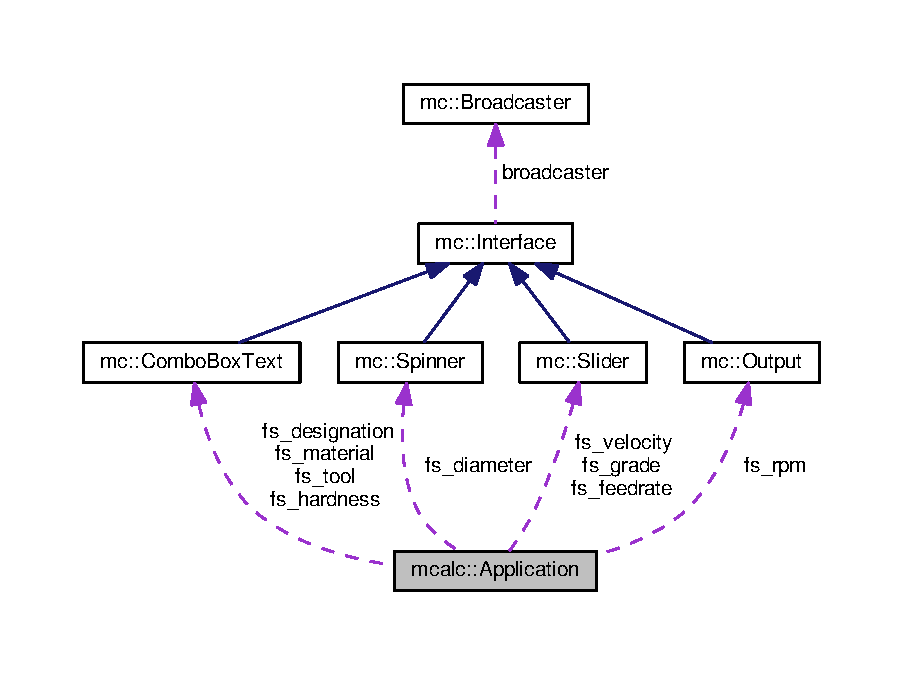
\includegraphics[width=350pt]{classmcalc_1_1Application__coll__graph}
\end{center}
\end{figure}
\subsection*{Public Member Functions}
\begin{DoxyCompactItemize}
\item 
\hyperlink{classmcalc_1_1Application_a44bc4c3091df2f37d9c5c5773d18de59}{Application} (Glib\+::\+Ref\+Ptr$<$ Gtk\+::\+Builder $>$ b, \hyperlink{application_8hpp_ab701e3ac61a85b337ec5c1abaad6742d}{json} d)
\item 
\hyperlink{classmcalc_1_1Application_a74e71090e2ccb489e865fd55875c36bf}{$\sim$\+Application} ()
\item 
{\footnotesize template$<$class A , class B $>$ }\\A $\ast$ \hyperlink{classmcalc_1_1Application_a11b823b5d31e917b83e97806bcbbcb18}{get\+\_\+wrapper} (std\+::string n)
\end{DoxyCompactItemize}
\subsection*{Protected Attributes}
\begin{DoxyCompactItemize}
\item 
Glib\+::\+Ref\+Ptr$<$ Gtk\+::\+Builder $>$ \hyperlink{classmcalc_1_1Application_ae877f6c9210ec88c743a54f750a54892}{builder}
\item 
\hyperlink{application_8hpp_ab701e3ac61a85b337ec5c1abaad6742d}{json} \hyperlink{classmcalc_1_1Application_a2fa9d06d424a8def5ea70fa07e844b9c}{datastore}
\item 
\hyperlink{classmc_1_1ComboBoxText}{mc\+::\+Combo\+Box\+Text} $\ast$ \hyperlink{classmcalc_1_1Application_a8c78f8ea0615db28858001aa5ed6b7b6}{fs\+\_\+material}
\item 
\hyperlink{classmc_1_1ComboBoxText}{mc\+::\+Combo\+Box\+Text} $\ast$ \hyperlink{classmcalc_1_1Application_a5dd81c68d005acedeb18336bfe87cdcb}{fs\+\_\+designation}
\item 
\hyperlink{classmc_1_1ComboBoxText}{mc\+::\+Combo\+Box\+Text} $\ast$ \hyperlink{classmcalc_1_1Application_acf53945a5bd5386c2d492e225878c45c}{fs\+\_\+hardness}
\item 
\hyperlink{classmc_1_1ComboBoxText}{mc\+::\+Combo\+Box\+Text} $\ast$ \hyperlink{classmcalc_1_1Application_a9775057e24515e6e3cf8c1c9a3144512}{fs\+\_\+tool}
\item 
\hyperlink{classmc_1_1Spinner}{mc\+::\+Spinner} $\ast$ \hyperlink{classmcalc_1_1Application_aa5fa7c6a44d89abb85a6947767261698}{fs\+\_\+diameter}
\item 
\hyperlink{classmc_1_1Slider}{mc\+::\+Slider} $\ast$ \hyperlink{classmcalc_1_1Application_aa92847f0410356a5515c461b269a840d}{fs\+\_\+grade}
\item 
\hyperlink{classmc_1_1Slider}{mc\+::\+Slider} $\ast$ \hyperlink{classmcalc_1_1Application_a6d4441380476fcbdafe23b28da5f6647}{fs\+\_\+velocity}
\item 
\hyperlink{classmc_1_1Slider}{mc\+::\+Slider} $\ast$ \hyperlink{classmcalc_1_1Application_a7cd486d0bde1d1ecdf82c41a5f2e6d53}{fs\+\_\+feedrate}
\item 
\hyperlink{classmc_1_1Output}{mc\+::\+Output} $\ast$ \hyperlink{classmcalc_1_1Application_a4b08a214c34fcb417f5cd14ca2e479c0}{fs\+\_\+rpm}
\end{DoxyCompactItemize}


\subsection{Detailed Description}
The main application manager. Maintains the interface wrappers around individual G\+UI elements (Gtk\+::\+Widgets). 

\subsection{Constructor \& Destructor Documentation}
\index{mcalc\+::\+Application@{mcalc\+::\+Application}!Application@{Application}}
\index{Application@{Application}!mcalc\+::\+Application@{mcalc\+::\+Application}}
\subsubsection[{\texorpdfstring{Application(\+Glib\+::\+Ref\+Ptr$<$ Gtk\+::\+Builder $>$ b, json d)}{Application(Glib::RefPtr< Gtk::Builder > b, json d)}}]{\setlength{\rightskip}{0pt plus 5cm}mcalc\+::\+Application\+::\+Application (
\begin{DoxyParamCaption}
\item[{Glib\+::\+Ref\+Ptr$<$ Gtk\+::\+Builder $>$}]{b, }
\item[{{\bf json}}]{d}
\end{DoxyParamCaption}
)}\hypertarget{classmcalc_1_1Application_a44bc4c3091df2f37d9c5c5773d18de59}{}\label{classmcalc_1_1Application_a44bc4c3091df2f37d9c5c5773d18de59}
The constructor for the application.


\begin{DoxyParams}{Parameters}
{\em b} & A Gtk\+::\+Builder initialized from a glade file. \\
\hline
{\em d} & J\+S\+ON data used for value lookups and populating the ui. \\
\hline
\end{DoxyParams}
\index{mcalc\+::\+Application@{mcalc\+::\+Application}!````~Application@{$\sim$\+Application}}
\index{````~Application@{$\sim$\+Application}!mcalc\+::\+Application@{mcalc\+::\+Application}}
\subsubsection[{\texorpdfstring{$\sim$\+Application()}{~Application()}}]{\setlength{\rightskip}{0pt plus 5cm}mcalc\+::\+Application\+::$\sim$\+Application (
\begin{DoxyParamCaption}
{}
\end{DoxyParamCaption}
)}\hypertarget{classmcalc_1_1Application_a74e71090e2ccb489e865fd55875c36bf}{}\label{classmcalc_1_1Application_a74e71090e2ccb489e865fd55875c36bf}
The application destructor 

\subsection{Member Function Documentation}
\index{mcalc\+::\+Application@{mcalc\+::\+Application}!get\+\_\+wrapper@{get\+\_\+wrapper}}
\index{get\+\_\+wrapper@{get\+\_\+wrapper}!mcalc\+::\+Application@{mcalc\+::\+Application}}
\subsubsection[{\texorpdfstring{get\+\_\+wrapper(std\+::string n)}{get_wrapper(std::string n)}}]{\setlength{\rightskip}{0pt plus 5cm}template$<$class A , class B $>$ A $\ast$ mcalc\+::\+Application\+::get\+\_\+wrapper (
\begin{DoxyParamCaption}
\item[{std\+::string}]{n}
\end{DoxyParamCaption}
)}\hypertarget{classmcalc_1_1Application_a11b823b5d31e917b83e97806bcbbcb18}{}\label{classmcalc_1_1Application_a11b823b5d31e917b83e97806bcbbcb18}
A templated function that generates Interfaces for given Gtk\+::\+Widgets.


\begin{DoxyTemplParams}{Template Parameters}
{\em A} & The Interface subclass to create \\
\hline
{\em B} & The Gtk\+::\+Widget type to look up\\
\hline
\end{DoxyTemplParams}

\begin{DoxyParams}{Parameters}
{\em n} & The name to lookup in builder (Gtk\+::\+Builder) \\
\hline
\end{DoxyParams}
\begin{DoxyReturn}{Returns}
The new Interface object. 
\end{DoxyReturn}


\subsection{Member Data Documentation}
\index{mcalc\+::\+Application@{mcalc\+::\+Application}!builder@{builder}}
\index{builder@{builder}!mcalc\+::\+Application@{mcalc\+::\+Application}}
\subsubsection[{\texorpdfstring{builder}{builder}}]{\setlength{\rightskip}{0pt plus 5cm}Glib\+::\+Ref\+Ptr$<$Gtk\+::\+Builder$>$ mcalc\+::\+Application\+::builder\hspace{0.3cm}{\ttfamily [protected]}}\hypertarget{classmcalc_1_1Application_ae877f6c9210ec88c743a54f750a54892}{}\label{classmcalc_1_1Application_ae877f6c9210ec88c743a54f750a54892}
The Gtk\+::\+Builder that is used to fetch ui elements. \index{mcalc\+::\+Application@{mcalc\+::\+Application}!datastore@{datastore}}
\index{datastore@{datastore}!mcalc\+::\+Application@{mcalc\+::\+Application}}
\subsubsection[{\texorpdfstring{datastore}{datastore}}]{\setlength{\rightskip}{0pt plus 5cm}{\bf json} mcalc\+::\+Application\+::datastore\hspace{0.3cm}{\ttfamily [protected]}}\hypertarget{classmcalc_1_1Application_a2fa9d06d424a8def5ea70fa07e844b9c}{}\label{classmcalc_1_1Application_a2fa9d06d424a8def5ea70fa07e844b9c}
The generated tabls and other data used for lookups. \index{mcalc\+::\+Application@{mcalc\+::\+Application}!fs\+\_\+designation@{fs\+\_\+designation}}
\index{fs\+\_\+designation@{fs\+\_\+designation}!mcalc\+::\+Application@{mcalc\+::\+Application}}
\subsubsection[{\texorpdfstring{fs\+\_\+designation}{fs_designation}}]{\setlength{\rightskip}{0pt plus 5cm}{\bf mc\+::\+Combo\+Box\+Text}$\ast$ mcalc\+::\+Application\+::fs\+\_\+designation\hspace{0.3cm}{\ttfamily [protected]}}\hypertarget{classmcalc_1_1Application_a5dd81c68d005acedeb18336bfe87cdcb}{}\label{classmcalc_1_1Application_a5dd81c68d005acedeb18336bfe87cdcb}
A\+I\+S\+I/\+S\+AE material designation \index{mcalc\+::\+Application@{mcalc\+::\+Application}!fs\+\_\+diameter@{fs\+\_\+diameter}}
\index{fs\+\_\+diameter@{fs\+\_\+diameter}!mcalc\+::\+Application@{mcalc\+::\+Application}}
\subsubsection[{\texorpdfstring{fs\+\_\+diameter}{fs_diameter}}]{\setlength{\rightskip}{0pt plus 5cm}{\bf mc\+::\+Spinner}$\ast$ mcalc\+::\+Application\+::fs\+\_\+diameter\hspace{0.3cm}{\ttfamily [protected]}}\hypertarget{classmcalc_1_1Application_aa5fa7c6a44d89abb85a6947767261698}{}\label{classmcalc_1_1Application_aa5fa7c6a44d89abb85a6947767261698}
diameter of the material \index{mcalc\+::\+Application@{mcalc\+::\+Application}!fs\+\_\+feedrate@{fs\+\_\+feedrate}}
\index{fs\+\_\+feedrate@{fs\+\_\+feedrate}!mcalc\+::\+Application@{mcalc\+::\+Application}}
\subsubsection[{\texorpdfstring{fs\+\_\+feedrate}{fs_feedrate}}]{\setlength{\rightskip}{0pt plus 5cm}{\bf mc\+::\+Slider}$\ast$ mcalc\+::\+Application\+::fs\+\_\+feedrate\hspace{0.3cm}{\ttfamily [protected]}}\hypertarget{classmcalc_1_1Application_a7cd486d0bde1d1ecdf82c41a5f2e6d53}{}\label{classmcalc_1_1Application_a7cd486d0bde1d1ecdf82c41a5f2e6d53}
feed rate of material \index{mcalc\+::\+Application@{mcalc\+::\+Application}!fs\+\_\+grade@{fs\+\_\+grade}}
\index{fs\+\_\+grade@{fs\+\_\+grade}!mcalc\+::\+Application@{mcalc\+::\+Application}}
\subsubsection[{\texorpdfstring{fs\+\_\+grade}{fs_grade}}]{\setlength{\rightskip}{0pt plus 5cm}{\bf mc\+::\+Slider}$\ast$ mcalc\+::\+Application\+::fs\+\_\+grade\hspace{0.3cm}{\ttfamily [protected]}}\hypertarget{classmcalc_1_1Application_aa92847f0410356a5515c461b269a840d}{}\label{classmcalc_1_1Application_aa92847f0410356a5515c461b269a840d}
grade of material (hard/tough) \index{mcalc\+::\+Application@{mcalc\+::\+Application}!fs\+\_\+hardness@{fs\+\_\+hardness}}
\index{fs\+\_\+hardness@{fs\+\_\+hardness}!mcalc\+::\+Application@{mcalc\+::\+Application}}
\subsubsection[{\texorpdfstring{fs\+\_\+hardness}{fs_hardness}}]{\setlength{\rightskip}{0pt plus 5cm}{\bf mc\+::\+Combo\+Box\+Text}$\ast$ mcalc\+::\+Application\+::fs\+\_\+hardness\hspace{0.3cm}{\ttfamily [protected]}}\hypertarget{classmcalc_1_1Application_acf53945a5bd5386c2d492e225878c45c}{}\label{classmcalc_1_1Application_acf53945a5bd5386c2d492e225878c45c}
material hardness \index{mcalc\+::\+Application@{mcalc\+::\+Application}!fs\+\_\+material@{fs\+\_\+material}}
\index{fs\+\_\+material@{fs\+\_\+material}!mcalc\+::\+Application@{mcalc\+::\+Application}}
\subsubsection[{\texorpdfstring{fs\+\_\+material}{fs_material}}]{\setlength{\rightskip}{0pt plus 5cm}{\bf mc\+::\+Combo\+Box\+Text}$\ast$ mcalc\+::\+Application\+::fs\+\_\+material\hspace{0.3cm}{\ttfamily [protected]}}\hypertarget{classmcalc_1_1Application_a8c78f8ea0615db28858001aa5ed6b7b6}{}\label{classmcalc_1_1Application_a8c78f8ea0615db28858001aa5ed6b7b6}
material to use \index{mcalc\+::\+Application@{mcalc\+::\+Application}!fs\+\_\+rpm@{fs\+\_\+rpm}}
\index{fs\+\_\+rpm@{fs\+\_\+rpm}!mcalc\+::\+Application@{mcalc\+::\+Application}}
\subsubsection[{\texorpdfstring{fs\+\_\+rpm}{fs_rpm}}]{\setlength{\rightskip}{0pt plus 5cm}{\bf mc\+::\+Output}$\ast$ mcalc\+::\+Application\+::fs\+\_\+rpm\hspace{0.3cm}{\ttfamily [protected]}}\hypertarget{classmcalc_1_1Application_a4b08a214c34fcb417f5cd14ca2e479c0}{}\label{classmcalc_1_1Application_a4b08a214c34fcb417f5cd14ca2e479c0}
revolutions per minute \index{mcalc\+::\+Application@{mcalc\+::\+Application}!fs\+\_\+tool@{fs\+\_\+tool}}
\index{fs\+\_\+tool@{fs\+\_\+tool}!mcalc\+::\+Application@{mcalc\+::\+Application}}
\subsubsection[{\texorpdfstring{fs\+\_\+tool}{fs_tool}}]{\setlength{\rightskip}{0pt plus 5cm}{\bf mc\+::\+Combo\+Box\+Text}$\ast$ mcalc\+::\+Application\+::fs\+\_\+tool\hspace{0.3cm}{\ttfamily [protected]}}\hypertarget{classmcalc_1_1Application_a9775057e24515e6e3cf8c1c9a3144512}{}\label{classmcalc_1_1Application_a9775057e24515e6e3cf8c1c9a3144512}
cutting tool to use \index{mcalc\+::\+Application@{mcalc\+::\+Application}!fs\+\_\+velocity@{fs\+\_\+velocity}}
\index{fs\+\_\+velocity@{fs\+\_\+velocity}!mcalc\+::\+Application@{mcalc\+::\+Application}}
\subsubsection[{\texorpdfstring{fs\+\_\+velocity}{fs_velocity}}]{\setlength{\rightskip}{0pt plus 5cm}{\bf mc\+::\+Slider}$\ast$ mcalc\+::\+Application\+::fs\+\_\+velocity\hspace{0.3cm}{\ttfamily [protected]}}\hypertarget{classmcalc_1_1Application_a6d4441380476fcbdafe23b28da5f6647}{}\label{classmcalc_1_1Application_a6d4441380476fcbdafe23b28da5f6647}
speed of the tool 

The documentation for this class was generated from the following files\+:\begin{DoxyCompactItemize}
\item 
inc/\hyperlink{application_8hpp}{application.\+hpp}\item 
src/application.\+cpp\end{DoxyCompactItemize}

\hypertarget{classmc_1_1Broadcaster}{}\section{mc\+:\+:Broadcaster Class Reference}
\label{classmc_1_1Broadcaster}\index{mc\+::\+Broadcaster@{mc\+::\+Broadcaster}}


{\ttfamily \#include $<$broadcaster.\+hpp$>$}

\subsection*{Public Member Functions}
\begin{DoxyCompactItemize}
\item 
\hyperlink{classmc_1_1Broadcaster_a300986f66a31e98e6d539cf0f47ad826}{$\sim$\+Broadcaster} ()
\item 
void \hyperlink{classmc_1_1Broadcaster_aad912e54f0309b68f32fe1cd40e4abb5}{subscribe} (\hyperlink{classmc_1_1Interface}{Interface} $\ast$s)
\item 
void \hyperlink{classmc_1_1Broadcaster_a7779ed0c085d890e1a25af4f104bf8cc}{broadcast} (\hyperlink{classmc_1_1Event}{Event} e)
\end{DoxyCompactItemize}
\subsection*{Static Public Member Functions}
\begin{DoxyCompactItemize}
\item 
static \hyperlink{classmc_1_1Broadcaster}{Broadcaster} $\ast$ \hyperlink{classmc_1_1Broadcaster_a2f5d57c051b9dd3132529f79de43d178}{get\+\_\+instance} ()
\end{DoxyCompactItemize}


\subsection{Detailed Description}
The \hyperlink{classmc_1_1Broadcaster}{Broadcaster} singleton class that acts as a communication channel for Interfaces. 

\subsection{Constructor \& Destructor Documentation}
\index{mc\+::\+Broadcaster@{mc\+::\+Broadcaster}!````~Broadcaster@{$\sim$\+Broadcaster}}
\index{````~Broadcaster@{$\sim$\+Broadcaster}!mc\+::\+Broadcaster@{mc\+::\+Broadcaster}}
\subsubsection[{\texorpdfstring{$\sim$\+Broadcaster()}{~Broadcaster()}}]{\setlength{\rightskip}{0pt plus 5cm}mc\+::\+Broadcaster\+::$\sim$\+Broadcaster (
\begin{DoxyParamCaption}
{}
\end{DoxyParamCaption}
)}\hypertarget{classmc_1_1Broadcaster_a300986f66a31e98e6d539cf0f47ad826}{}\label{classmc_1_1Broadcaster_a300986f66a31e98e6d539cf0f47ad826}
The destructor 

\subsection{Member Function Documentation}
\index{mc\+::\+Broadcaster@{mc\+::\+Broadcaster}!broadcast@{broadcast}}
\index{broadcast@{broadcast}!mc\+::\+Broadcaster@{mc\+::\+Broadcaster}}
\subsubsection[{\texorpdfstring{broadcast(\+Event e)}{broadcast(Event e)}}]{\setlength{\rightskip}{0pt plus 5cm}void mc\+::\+Broadcaster\+::broadcast (
\begin{DoxyParamCaption}
\item[{{\bf Event}}]{e}
\end{DoxyParamCaption}
)}\hypertarget{classmc_1_1Broadcaster_a7779ed0c085d890e1a25af4f104bf8cc}{}\label{classmc_1_1Broadcaster_a7779ed0c085d890e1a25af4f104bf8cc}
Broadcast an event to all subscribed interfaces \index{mc\+::\+Broadcaster@{mc\+::\+Broadcaster}!get\+\_\+instance@{get\+\_\+instance}}
\index{get\+\_\+instance@{get\+\_\+instance}!mc\+::\+Broadcaster@{mc\+::\+Broadcaster}}
\subsubsection[{\texorpdfstring{get\+\_\+instance()}{get_instance()}}]{\setlength{\rightskip}{0pt plus 5cm}{\bf Broadcaster} $\ast$ mc\+::\+Broadcaster\+::get\+\_\+instance (
\begin{DoxyParamCaption}
{}
\end{DoxyParamCaption}
)\hspace{0.3cm}{\ttfamily [static]}}\hypertarget{classmc_1_1Broadcaster_a2f5d57c051b9dd3132529f79de43d178}{}\label{classmc_1_1Broadcaster_a2f5d57c051b9dd3132529f79de43d178}
Get the singleton instance of broadcaster \index{mc\+::\+Broadcaster@{mc\+::\+Broadcaster}!subscribe@{subscribe}}
\index{subscribe@{subscribe}!mc\+::\+Broadcaster@{mc\+::\+Broadcaster}}
\subsubsection[{\texorpdfstring{subscribe(\+Interface $\ast$s)}{subscribe(Interface *s)}}]{\setlength{\rightskip}{0pt plus 5cm}void mc\+::\+Broadcaster\+::subscribe (
\begin{DoxyParamCaption}
\item[{{\bf Interface} $\ast$}]{s}
\end{DoxyParamCaption}
)}\hypertarget{classmc_1_1Broadcaster_aad912e54f0309b68f32fe1cd40e4abb5}{}\label{classmc_1_1Broadcaster_aad912e54f0309b68f32fe1cd40e4abb5}
Subscribe an interface to receive notifications 

The documentation for this class was generated from the following files\+:\begin{DoxyCompactItemize}
\item 
inc/\hyperlink{broadcaster_8hpp}{broadcaster.\+hpp}\item 
src/broadcaster.\+cpp\end{DoxyCompactItemize}

\hypertarget{classmc_1_1ComboBoxText}{}\section{mc\+:\+:Combo\+Box\+Text Class Reference}
\label{classmc_1_1ComboBoxText}\index{mc\+::\+Combo\+Box\+Text@{mc\+::\+Combo\+Box\+Text}}


{\ttfamily \#include $<$comboboxtext.\+hpp$>$}



Inheritance diagram for mc\+:\+:Combo\+Box\+Text\+:\nopagebreak
\begin{figure}[H]
\begin{center}
\leavevmode
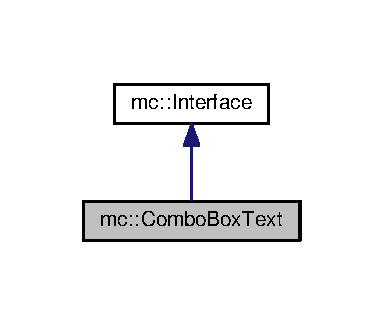
\includegraphics[width=184pt]{classmc_1_1ComboBoxText__inherit__graph}
\end{center}
\end{figure}


Collaboration diagram for mc\+:\+:Combo\+Box\+Text\+:\nopagebreak
\begin{figure}[H]
\begin{center}
\leavevmode
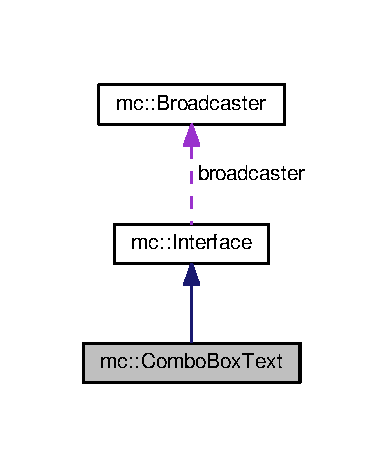
\includegraphics[width=187pt]{classmc_1_1ComboBoxText__coll__graph}
\end{center}
\end{figure}
\subsection*{Public Member Functions}
\begin{DoxyCompactItemize}
\item 
\hyperlink{classmc_1_1ComboBoxText_a1131fdddb8a549ff4cac54d8b58ffad8}{Combo\+Box\+Text} (Gtk\+::\+Combo\+Box\+Text $\ast$w, \hyperlink{application_8hpp_ab701e3ac61a85b337ec5c1abaad6742d}{json} $\ast$d)
\item 
\hyperlink{classmc_1_1ComboBoxText_a87084073a37ee5e34852b4e2fd539195}{$\sim$\+Combo\+Box\+Text} ()
\item 
void \hyperlink{classmc_1_1ComboBoxText_acc725c32e20e84062c31fdb7b522f61b}{notify} (\hyperlink{classmc_1_1Event}{Event} $\ast$e)
\item 
void \hyperlink{classmc_1_1ComboBoxText_aef38e11777ac04e0b91c709eddbf3197}{broadcast} ()
\item 
void \hyperlink{classmc_1_1ComboBoxText_acac1e8f7b02c7cc76098768c6bcf9d12}{populate} ()
\item 
void \hyperlink{classmc_1_1ComboBoxText_af140937525bfd17e74a7786a24f086bb}{set\+\_\+references} (std\+::vector$<$ \hyperlink{classmc_1_1Interface}{Interface} $\ast$ $>$ i)
\item 
std\+::string \hyperlink{classmc_1_1ComboBoxText_a38664e490a06e3976aeefe6e69896df3}{get\+\_\+value} ()
\item 
void \hyperlink{classmc_1_1ComboBoxText_a2e5eaed5544e2c320ec4b918f3bb9a59}{set\+\_\+value} (std\+::vector$<$ std\+::string $>$ v)
\end{DoxyCompactItemize}
\subsection*{Additional Inherited Members}


\subsection{Detailed Description}
\hyperlink{classmc_1_1ComboBoxText}{Combo\+Box\+Text} wraps a Gtk\+::\+Combo\+Box\+Text widget, updates it when dependent values change, and broadcasts an event when the user selects a value. 

\subsection{Constructor \& Destructor Documentation}
\index{mc\+::\+Combo\+Box\+Text@{mc\+::\+Combo\+Box\+Text}!Combo\+Box\+Text@{Combo\+Box\+Text}}
\index{Combo\+Box\+Text@{Combo\+Box\+Text}!mc\+::\+Combo\+Box\+Text@{mc\+::\+Combo\+Box\+Text}}
\subsubsection[{\texorpdfstring{Combo\+Box\+Text(\+Gtk\+::\+Combo\+Box\+Text $\ast$w, json $\ast$d)}{ComboBoxText(Gtk::ComboBoxText *w, json *d)}}]{\setlength{\rightskip}{0pt plus 5cm}mc\+::\+Combo\+Box\+Text\+::\+Combo\+Box\+Text (
\begin{DoxyParamCaption}
\item[{Gtk\+::\+Combo\+Box\+Text $\ast$}]{w, }
\item[{{\bf json} $\ast$}]{d}
\end{DoxyParamCaption}
)}\hypertarget{classmc_1_1ComboBoxText_a1131fdddb8a549ff4cac54d8b58ffad8}{}\label{classmc_1_1ComboBoxText_a1131fdddb8a549ff4cac54d8b58ffad8}
Constructor 
\begin{DoxyParams}{Parameters}
{\em w} & the Gtk\+::\+Combo\+Box\+Text to wrap \\
\hline
{\em d} & Pointer to the json datastore \\
\hline
\end{DoxyParams}
\index{mc\+::\+Combo\+Box\+Text@{mc\+::\+Combo\+Box\+Text}!````~Combo\+Box\+Text@{$\sim$\+Combo\+Box\+Text}}
\index{````~Combo\+Box\+Text@{$\sim$\+Combo\+Box\+Text}!mc\+::\+Combo\+Box\+Text@{mc\+::\+Combo\+Box\+Text}}
\subsubsection[{\texorpdfstring{$\sim$\+Combo\+Box\+Text()}{~ComboBoxText()}}]{\setlength{\rightskip}{0pt plus 5cm}mc\+::\+Combo\+Box\+Text\+::$\sim$\+Combo\+Box\+Text (
\begin{DoxyParamCaption}
{}
\end{DoxyParamCaption}
)}\hypertarget{classmc_1_1ComboBoxText_a87084073a37ee5e34852b4e2fd539195}{}\label{classmc_1_1ComboBoxText_a87084073a37ee5e34852b4e2fd539195}
The destructor 

\subsection{Member Function Documentation}
\index{mc\+::\+Combo\+Box\+Text@{mc\+::\+Combo\+Box\+Text}!broadcast@{broadcast}}
\index{broadcast@{broadcast}!mc\+::\+Combo\+Box\+Text@{mc\+::\+Combo\+Box\+Text}}
\subsubsection[{\texorpdfstring{broadcast()}{broadcast()}}]{\setlength{\rightskip}{0pt plus 5cm}void mc\+::\+Combo\+Box\+Text\+::broadcast (
\begin{DoxyParamCaption}
{}
\end{DoxyParamCaption}
)\hspace{0.3cm}{\ttfamily [virtual]}}\hypertarget{classmc_1_1ComboBoxText_aef38e11777ac04e0b91c709eddbf3197}{}\label{classmc_1_1ComboBoxText_aef38e11777ac04e0b91c709eddbf3197}
Sends out a change event. 

Implements \hyperlink{classmc_1_1Interface_af91ff5ec779e5af49bf798d5f6331b80}{mc\+::\+Interface}.

\index{mc\+::\+Combo\+Box\+Text@{mc\+::\+Combo\+Box\+Text}!get\+\_\+value@{get\+\_\+value}}
\index{get\+\_\+value@{get\+\_\+value}!mc\+::\+Combo\+Box\+Text@{mc\+::\+Combo\+Box\+Text}}
\subsubsection[{\texorpdfstring{get\+\_\+value()}{get_value()}}]{\setlength{\rightskip}{0pt plus 5cm}std\+::string mc\+::\+Combo\+Box\+Text\+::get\+\_\+value (
\begin{DoxyParamCaption}
{}
\end{DoxyParamCaption}
)\hspace{0.3cm}{\ttfamily [virtual]}}\hypertarget{classmc_1_1ComboBoxText_a38664e490a06e3976aeefe6e69896df3}{}\label{classmc_1_1ComboBoxText_a38664e490a06e3976aeefe6e69896df3}
Get the current value of the \hyperlink{classmc_1_1ComboBoxText}{Combo\+Box\+Text} 

Implements \hyperlink{classmc_1_1Interface_af8054c8af251199c9d142ce94182c5f5}{mc\+::\+Interface}.

\index{mc\+::\+Combo\+Box\+Text@{mc\+::\+Combo\+Box\+Text}!notify@{notify}}
\index{notify@{notify}!mc\+::\+Combo\+Box\+Text@{mc\+::\+Combo\+Box\+Text}}
\subsubsection[{\texorpdfstring{notify(\+Event $\ast$e)}{notify(Event *e)}}]{\setlength{\rightskip}{0pt plus 5cm}void mc\+::\+Combo\+Box\+Text\+::notify (
\begin{DoxyParamCaption}
\item[{{\bf Event} $\ast$}]{e}
\end{DoxyParamCaption}
)\hspace{0.3cm}{\ttfamily [virtual]}}\hypertarget{classmc_1_1ComboBoxText_acc725c32e20e84062c31fdb7b522f61b}{}\label{classmc_1_1ComboBoxText_acc725c32e20e84062c31fdb7b522f61b}
Method used to update the \hyperlink{classmc_1_1ComboBoxText}{Combo\+Box\+Text} by the broadcaster. 
\begin{DoxyParams}{Parameters}
{\em e} & \hyperlink{classmc_1_1Event}{Event} received from broadcaster \\
\hline
\end{DoxyParams}


Implements \hyperlink{classmc_1_1Interface_a6a08326bd2ad5d40fe0427e97cebfbb6}{mc\+::\+Interface}.

\index{mc\+::\+Combo\+Box\+Text@{mc\+::\+Combo\+Box\+Text}!populate@{populate}}
\index{populate@{populate}!mc\+::\+Combo\+Box\+Text@{mc\+::\+Combo\+Box\+Text}}
\subsubsection[{\texorpdfstring{populate()}{populate()}}]{\setlength{\rightskip}{0pt plus 5cm}void mc\+::\+Combo\+Box\+Text\+::populate (
\begin{DoxyParamCaption}
{}
\end{DoxyParamCaption}
)}\hypertarget{classmc_1_1ComboBoxText_acac1e8f7b02c7cc76098768c6bcf9d12}{}\label{classmc_1_1ComboBoxText_acac1e8f7b02c7cc76098768c6bcf9d12}
Populates the UI with values from the datastore. \index{mc\+::\+Combo\+Box\+Text@{mc\+::\+Combo\+Box\+Text}!set\+\_\+references@{set\+\_\+references}}
\index{set\+\_\+references@{set\+\_\+references}!mc\+::\+Combo\+Box\+Text@{mc\+::\+Combo\+Box\+Text}}
\subsubsection[{\texorpdfstring{set\+\_\+references(std\+::vector$<$ Interface $\ast$ $>$ i)}{set_references(std::vector< Interface * > i)}}]{\setlength{\rightskip}{0pt plus 5cm}void mc\+::\+Combo\+Box\+Text\+::set\+\_\+references (
\begin{DoxyParamCaption}
\item[{std\+::vector$<$ {\bf Interface} $\ast$ $>$}]{i}
\end{DoxyParamCaption}
)}\hypertarget{classmc_1_1ComboBoxText_af140937525bfd17e74a7786a24f086bb}{}\label{classmc_1_1ComboBoxText_af140937525bfd17e74a7786a24f086bb}
Add references to the interface that will trigger the \hyperlink{classmc_1_1ComboBoxText}{Combo\+Box\+Text} to update when they change. 
\begin{DoxyParams}{Parameters}
{\em i} & A vector of Interfaces to use as a reference \\
\hline
\end{DoxyParams}
\index{mc\+::\+Combo\+Box\+Text@{mc\+::\+Combo\+Box\+Text}!set\+\_\+value@{set\+\_\+value}}
\index{set\+\_\+value@{set\+\_\+value}!mc\+::\+Combo\+Box\+Text@{mc\+::\+Combo\+Box\+Text}}
\subsubsection[{\texorpdfstring{set\+\_\+value(std\+::vector$<$ std\+::string $>$ v)}{set_value(std::vector< std::string > v)}}]{\setlength{\rightskip}{0pt plus 5cm}void mc\+::\+Combo\+Box\+Text\+::set\+\_\+value (
\begin{DoxyParamCaption}
\item[{std\+::vector$<$ std\+::string $>$}]{v}
\end{DoxyParamCaption}
)}\hypertarget{classmc_1_1ComboBoxText_a2e5eaed5544e2c320ec4b918f3bb9a59}{}\label{classmc_1_1ComboBoxText_a2e5eaed5544e2c320ec4b918f3bb9a59}
Set the \hyperlink{classmc_1_1ComboBoxText}{Combo\+Box\+Text} contents 
\begin{DoxyParams}{Parameters}
{\em v} & A vector of strings to use as entries \\
\hline
\end{DoxyParams}


The documentation for this class was generated from the following files\+:\begin{DoxyCompactItemize}
\item 
inc/\hyperlink{comboboxtext_8hpp}{comboboxtext.\+hpp}\item 
src/comboboxtext.\+cpp\end{DoxyCompactItemize}

\hypertarget{classmc_1_1DummyInterface}{}\section{mc\+:\+:Dummy\+Interface Class Reference}
\label{classmc_1_1DummyInterface}\index{mc\+::\+Dummy\+Interface@{mc\+::\+Dummy\+Interface}}


{\ttfamily \#include $<$interface.\+hpp$>$}



Inheritance diagram for mc\+:\+:Dummy\+Interface\+:\nopagebreak
\begin{figure}[H]
\begin{center}
\leavevmode
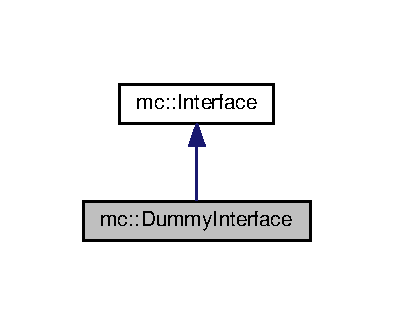
\includegraphics[width=189pt]{classmc_1_1DummyInterface__inherit__graph}
\end{center}
\end{figure}


Collaboration diagram for mc\+:\+:Dummy\+Interface\+:\nopagebreak
\begin{figure}[H]
\begin{center}
\leavevmode
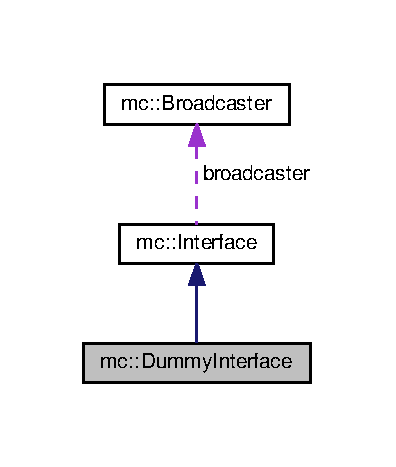
\includegraphics[width=190pt]{classmc_1_1DummyInterface__coll__graph}
\end{center}
\end{figure}
\subsection*{Public Member Functions}
\begin{DoxyCompactItemize}
\item 
\hyperlink{classmc_1_1DummyInterface_aa324d9b7a8dec1b074cda89490910ee3}{Dummy\+Interface} (std\+::string s)
\item 
std\+::string \hyperlink{classmc_1_1DummyInterface_a228a5d03c2a03bcd4c2a9890ed9271b4}{get\+\_\+value} ()
\item 
void \hyperlink{classmc_1_1DummyInterface_a75b062a80715ae9662342b48502318c2}{notify} (\hyperlink{classmc_1_1Event}{Event} $\ast$e)
\item 
void \hyperlink{classmc_1_1DummyInterface_a9a1b7d734f4da3fa360231921aa248b8}{broadcast} ()
\end{DoxyCompactItemize}
\subsection*{Additional Inherited Members}


\subsection{Detailed Description}
An empty implementation of \hyperlink{classmc_1_1Interface}{Interface} that wraps a constant string value. Used for plugging gaps in a path in the datastore when there isn\textquotesingle{}t a UI element for the value. 

\subsection{Constructor \& Destructor Documentation}
\index{mc\+::\+Dummy\+Interface@{mc\+::\+Dummy\+Interface}!Dummy\+Interface@{Dummy\+Interface}}
\index{Dummy\+Interface@{Dummy\+Interface}!mc\+::\+Dummy\+Interface@{mc\+::\+Dummy\+Interface}}
\subsubsection[{\texorpdfstring{Dummy\+Interface(std\+::string s)}{DummyInterface(std::string s)}}]{\setlength{\rightskip}{0pt plus 5cm}mc\+::\+Dummy\+Interface\+::\+Dummy\+Interface (
\begin{DoxyParamCaption}
\item[{std\+::string}]{s}
\end{DoxyParamCaption}
)\hspace{0.3cm}{\ttfamily [inline]}}\hypertarget{classmc_1_1DummyInterface_aa324d9b7a8dec1b074cda89490910ee3}{}\label{classmc_1_1DummyInterface_aa324d9b7a8dec1b074cda89490910ee3}
Constructor sets the value of the \hyperlink{classmc_1_1Interface}{Interface}. 
\begin{DoxyParams}{Parameters}
{\em s} & The constant value to use. \\
\hline
\end{DoxyParams}


\subsection{Member Function Documentation}
\index{mc\+::\+Dummy\+Interface@{mc\+::\+Dummy\+Interface}!broadcast@{broadcast}}
\index{broadcast@{broadcast}!mc\+::\+Dummy\+Interface@{mc\+::\+Dummy\+Interface}}
\subsubsection[{\texorpdfstring{broadcast()}{broadcast()}}]{\setlength{\rightskip}{0pt plus 5cm}void mc\+::\+Dummy\+Interface\+::broadcast (
\begin{DoxyParamCaption}
{}
\end{DoxyParamCaption}
)\hspace{0.3cm}{\ttfamily [inline]}, {\ttfamily [virtual]}}\hypertarget{classmc_1_1DummyInterface_a9a1b7d734f4da3fa360231921aa248b8}{}\label{classmc_1_1DummyInterface_a9a1b7d734f4da3fa360231921aa248b8}
Generates a change event and sends it to \hyperlink{classmc_1_1Broadcaster}{Broadcaster}. 

Implements \hyperlink{classmc_1_1Interface_af91ff5ec779e5af49bf798d5f6331b80}{mc\+::\+Interface}.

\index{mc\+::\+Dummy\+Interface@{mc\+::\+Dummy\+Interface}!get\+\_\+value@{get\+\_\+value}}
\index{get\+\_\+value@{get\+\_\+value}!mc\+::\+Dummy\+Interface@{mc\+::\+Dummy\+Interface}}
\subsubsection[{\texorpdfstring{get\+\_\+value()}{get_value()}}]{\setlength{\rightskip}{0pt plus 5cm}std\+::string mc\+::\+Dummy\+Interface\+::get\+\_\+value (
\begin{DoxyParamCaption}
{}
\end{DoxyParamCaption}
)\hspace{0.3cm}{\ttfamily [inline]}, {\ttfamily [virtual]}}\hypertarget{classmc_1_1DummyInterface_a228a5d03c2a03bcd4c2a9890ed9271b4}{}\label{classmc_1_1DummyInterface_a228a5d03c2a03bcd4c2a9890ed9271b4}
Returns a string representation of the current value of the \hyperlink{classmc_1_1Interface}{Interface}. 

Implements \hyperlink{classmc_1_1Interface_af8054c8af251199c9d142ce94182c5f5}{mc\+::\+Interface}.

\index{mc\+::\+Dummy\+Interface@{mc\+::\+Dummy\+Interface}!notify@{notify}}
\index{notify@{notify}!mc\+::\+Dummy\+Interface@{mc\+::\+Dummy\+Interface}}
\subsubsection[{\texorpdfstring{notify(\+Event $\ast$e)}{notify(Event *e)}}]{\setlength{\rightskip}{0pt plus 5cm}void mc\+::\+Dummy\+Interface\+::notify (
\begin{DoxyParamCaption}
\item[{{\bf Event} $\ast$}]{e}
\end{DoxyParamCaption}
)\hspace{0.3cm}{\ttfamily [inline]}, {\ttfamily [virtual]}}\hypertarget{classmc_1_1DummyInterface_a75b062a80715ae9662342b48502318c2}{}\label{classmc_1_1DummyInterface_a75b062a80715ae9662342b48502318c2}
Update the \hyperlink{classmc_1_1Interface}{Interface} about change events. Used by broadcaster. 
\begin{DoxyParams}{Parameters}
{\em e} & The event object \\
\hline
\end{DoxyParams}


Implements \hyperlink{classmc_1_1Interface_a6a08326bd2ad5d40fe0427e97cebfbb6}{mc\+::\+Interface}.



The documentation for this class was generated from the following file\+:\begin{DoxyCompactItemize}
\item 
inc/\hyperlink{interface_8hpp}{interface.\+hpp}\end{DoxyCompactItemize}

\hypertarget{classmc_1_1Event}{}\section{mc\+:\+:Event Class Reference}
\label{classmc_1_1Event}\index{mc\+::\+Event@{mc\+::\+Event}}


{\ttfamily \#include $<$broadcaster.\+hpp$>$}

\subsection*{Public Types}
\begin{DoxyCompactItemize}
\item 
enum \hyperlink{classmc_1_1Event_afe30211c7b3a7564272ed756e96c8717}{Type} \{ {\bfseries A\+LL}, 
{\bfseries S\+I\+N\+G\+LE}
 \}
\end{DoxyCompactItemize}
\subsection*{Public Member Functions}
\begin{DoxyCompactItemize}
\item 
\hyperlink{classmc_1_1Event_a1f2a094035fb1393bb3d7c9f3c6a604e}{Event} (\hyperlink{classmc_1_1Event_afe30211c7b3a7564272ed756e96c8717}{Type} t)
\item 
\hyperlink{classmc_1_1Event_a8ec8d92673d38611264a357d959beb08}{Event} (\hyperlink{classmc_1_1Interface}{Interface} $\ast$s)
\item 
\hyperlink{classmc_1_1Event_a14f5222905775d873f7da210b05907a4}{Event} (\hyperlink{classmc_1_1Event_afe30211c7b3a7564272ed756e96c8717}{Type} t, \hyperlink{classmc_1_1Interface}{Interface} $\ast$s)
\item 
\hyperlink{classmc_1_1Event_affe2c3084bf256be3c56789fdeb82567}{$\sim$\+Event} ()
\item 
\hyperlink{classmc_1_1Event_afe30211c7b3a7564272ed756e96c8717}{Event\+::\+Type} \hyperlink{classmc_1_1Event_ae95c0cc6d4609bb6c032c124caafbf4f}{type} ()
\item 
\hyperlink{classmc_1_1Interface}{Interface} $\ast$ \hyperlink{classmc_1_1Event_a05c4a8a5a5df79804315306dc1b6c257}{sender} ()
\end{DoxyCompactItemize}


\subsection{Detailed Description}
Events maintain an event type and a pointer to the sender who produced the event. 

\subsection{Member Enumeration Documentation}
\index{mc\+::\+Event@{mc\+::\+Event}!Type@{Type}}
\index{Type@{Type}!mc\+::\+Event@{mc\+::\+Event}}
\subsubsection[{\texorpdfstring{Type}{Type}}]{\setlength{\rightskip}{0pt plus 5cm}enum {\bf mc\+::\+Event\+::\+Type}}\hypertarget{classmc_1_1Event_afe30211c7b3a7564272ed756e96c8717}{}\label{classmc_1_1Event_afe30211c7b3a7564272ed756e96c8717}
The type of the event instance 

\subsection{Constructor \& Destructor Documentation}
\index{mc\+::\+Event@{mc\+::\+Event}!Event@{Event}}
\index{Event@{Event}!mc\+::\+Event@{mc\+::\+Event}}
\subsubsection[{\texorpdfstring{Event(\+Type t)}{Event(Type t)}}]{\setlength{\rightskip}{0pt plus 5cm}mc\+::\+Event\+::\+Event (
\begin{DoxyParamCaption}
\item[{{\bf Type}}]{t}
\end{DoxyParamCaption}
)}\hypertarget{classmc_1_1Event_a1f2a094035fb1393bb3d7c9f3c6a604e}{}\label{classmc_1_1Event_a1f2a094035fb1393bb3d7c9f3c6a604e}
Constructor with no sender, defaults the sender to nullptr 
\begin{DoxyParams}{Parameters}
{\em t} & The type of the new event \\
\hline
\end{DoxyParams}
\index{mc\+::\+Event@{mc\+::\+Event}!Event@{Event}}
\index{Event@{Event}!mc\+::\+Event@{mc\+::\+Event}}
\subsubsection[{\texorpdfstring{Event(\+Interface $\ast$s)}{Event(Interface *s)}}]{\setlength{\rightskip}{0pt plus 5cm}mc\+::\+Event\+::\+Event (
\begin{DoxyParamCaption}
\item[{{\bf Interface} $\ast$}]{s}
\end{DoxyParamCaption}
)}\hypertarget{classmc_1_1Event_a8ec8d92673d38611264a357d959beb08}{}\label{classmc_1_1Event_a8ec8d92673d38611264a357d959beb08}
Constructor with no type, defaults the type to A\+LL 
\begin{DoxyParams}{Parameters}
{\em s} & The sender \\
\hline
\end{DoxyParams}
\index{mc\+::\+Event@{mc\+::\+Event}!Event@{Event}}
\index{Event@{Event}!mc\+::\+Event@{mc\+::\+Event}}
\subsubsection[{\texorpdfstring{Event(\+Type t, Interface $\ast$s)}{Event(Type t, Interface *s)}}]{\setlength{\rightskip}{0pt plus 5cm}mc\+::\+Event\+::\+Event (
\begin{DoxyParamCaption}
\item[{{\bf Type}}]{t, }
\item[{{\bf Interface} $\ast$}]{s}
\end{DoxyParamCaption}
)}\hypertarget{classmc_1_1Event_a14f5222905775d873f7da210b05907a4}{}\label{classmc_1_1Event_a14f5222905775d873f7da210b05907a4}
Constructor with both type and sender. 
\begin{DoxyParams}{Parameters}
{\em t} & The type of the new event \\
\hline
{\em s} & The sender \\
\hline
\end{DoxyParams}
\index{mc\+::\+Event@{mc\+::\+Event}!````~Event@{$\sim$\+Event}}
\index{````~Event@{$\sim$\+Event}!mc\+::\+Event@{mc\+::\+Event}}
\subsubsection[{\texorpdfstring{$\sim$\+Event()}{~Event()}}]{\setlength{\rightskip}{0pt plus 5cm}mc\+::\+Event\+::$\sim$\+Event (
\begin{DoxyParamCaption}
{}
\end{DoxyParamCaption}
)\hspace{0.3cm}{\ttfamily [inline]}}\hypertarget{classmc_1_1Event_affe2c3084bf256be3c56789fdeb82567}{}\label{classmc_1_1Event_affe2c3084bf256be3c56789fdeb82567}
The destructor 

\subsection{Member Function Documentation}
\index{mc\+::\+Event@{mc\+::\+Event}!sender@{sender}}
\index{sender@{sender}!mc\+::\+Event@{mc\+::\+Event}}
\subsubsection[{\texorpdfstring{sender()}{sender()}}]{\setlength{\rightskip}{0pt plus 5cm}{\bf Interface} $\ast$ mc\+::\+Event\+::sender (
\begin{DoxyParamCaption}
{}
\end{DoxyParamCaption}
)}\hypertarget{classmc_1_1Event_a05c4a8a5a5df79804315306dc1b6c257}{}\label{classmc_1_1Event_a05c4a8a5a5df79804315306dc1b6c257}
Get a pointer to the sender \begin{DoxyReturn}{Returns}
The \hyperlink{classmc_1_1Interface}{Interface} that generated the event 
\end{DoxyReturn}
\index{mc\+::\+Event@{mc\+::\+Event}!type@{type}}
\index{type@{type}!mc\+::\+Event@{mc\+::\+Event}}
\subsubsection[{\texorpdfstring{type()}{type()}}]{\setlength{\rightskip}{0pt plus 5cm}{\bf Event\+::\+Type} mc\+::\+Event\+::type (
\begin{DoxyParamCaption}
{}
\end{DoxyParamCaption}
)}\hypertarget{classmc_1_1Event_ae95c0cc6d4609bb6c032c124caafbf4f}{}\label{classmc_1_1Event_ae95c0cc6d4609bb6c032c124caafbf4f}
Get the type of the instance \begin{DoxyReturn}{Returns}
The type of \hyperlink{classmc_1_1Event}{Event} 
\end{DoxyReturn}


The documentation for this class was generated from the following files\+:\begin{DoxyCompactItemize}
\item 
inc/\hyperlink{broadcaster_8hpp}{broadcaster.\+hpp}\item 
src/broadcaster.\+cpp\end{DoxyCompactItemize}

\hypertarget{classmc_1_1Interface}{}\section{mc\+:\+:Interface Class Reference}
\label{classmc_1_1Interface}\index{mc\+::\+Interface@{mc\+::\+Interface}}


{\ttfamily \#include $<$interface.\+hpp$>$}



Inheritance diagram for mc\+:\+:Interface\+:\nopagebreak
\begin{figure}[H]
\begin{center}
\leavevmode
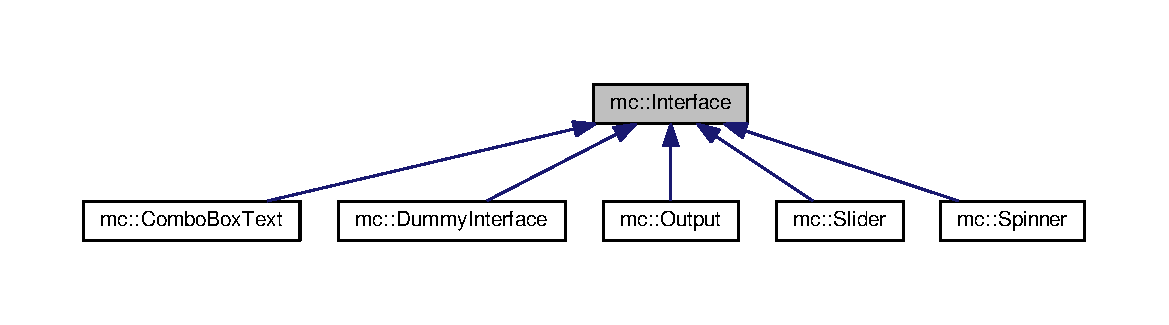
\includegraphics[width=350pt]{classmc_1_1Interface__inherit__graph}
\end{center}
\end{figure}


Collaboration diagram for mc\+:\+:Interface\+:\nopagebreak
\begin{figure}[H]
\begin{center}
\leavevmode
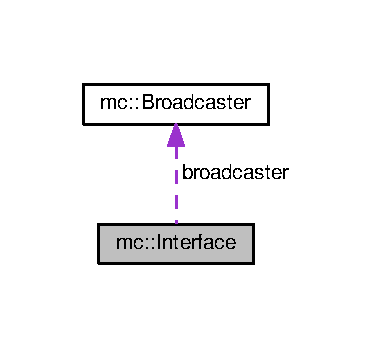
\includegraphics[width=180pt]{classmc_1_1Interface__coll__graph}
\end{center}
\end{figure}
\subsection*{Public Member Functions}
\begin{DoxyCompactItemize}
\item 
\hyperlink{classmc_1_1Interface_ad6af075feefe2afc9578724dd8ef2343}{Interface} ()
\item 
virtual \hyperlink{classmc_1_1Interface_a5d28302e778fd71f760cba7005b66b9f}{$\sim$\+Interface} ()
\item 
virtual std\+::string \hyperlink{classmc_1_1Interface_af8054c8af251199c9d142ce94182c5f5}{get\+\_\+value} ()=0
\item 
virtual void \hyperlink{classmc_1_1Interface_a6a08326bd2ad5d40fe0427e97cebfbb6}{notify} (\hyperlink{classmc_1_1Event}{Event} $\ast$e)=0
\item 
virtual void \hyperlink{classmc_1_1Interface_af91ff5ec779e5af49bf798d5f6331b80}{broadcast} ()=0
\end{DoxyCompactItemize}
\subsection*{Protected Member Functions}
\begin{DoxyCompactItemize}
\item 
\hyperlink{application_8hpp_ab701e3ac61a85b337ec5c1abaad6742d}{json} \hyperlink{classmc_1_1Interface_a231dc1d03130742787f2a16d2775a756}{tunnel} (\hyperlink{application_8hpp_ab701e3ac61a85b337ec5c1abaad6742d}{json} $\ast$d, std\+::vector$<$ \hyperlink{classmc_1_1Interface}{Interface} $\ast$ $>$ i)
\item 
std\+::vector$<$ double $>$ \hyperlink{classmc_1_1Interface_a552eca2a868f3de38a808a6b4da55985}{as\+\_\+vector} (\hyperlink{application_8hpp_ab701e3ac61a85b337ec5c1abaad6742d}{json} d)
\end{DoxyCompactItemize}
\subsection*{Protected Attributes}
\begin{DoxyCompactItemize}
\item 
\hyperlink{classmc_1_1Broadcaster}{Broadcaster} $\ast$ \hyperlink{classmc_1_1Interface_a7f56f04e9522f7b22076bc63327f5866}{broadcaster}
\end{DoxyCompactItemize}


\subsection{Detailed Description}
The abstract base class for Sliders, \hyperlink{classmc_1_1ComboBoxText}{Combo\+Box\+Text} etc. 

\subsection{Constructor \& Destructor Documentation}
\index{mc\+::\+Interface@{mc\+::\+Interface}!Interface@{Interface}}
\index{Interface@{Interface}!mc\+::\+Interface@{mc\+::\+Interface}}
\subsubsection[{\texorpdfstring{Interface()}{Interface()}}]{\setlength{\rightskip}{0pt plus 5cm}mc\+::\+Interface\+::\+Interface (
\begin{DoxyParamCaption}
{}
\end{DoxyParamCaption}
)}\hypertarget{classmc_1_1Interface_ad6af075feefe2afc9578724dd8ef2343}{}\label{classmc_1_1Interface_ad6af075feefe2afc9578724dd8ef2343}
Constructor \index{mc\+::\+Interface@{mc\+::\+Interface}!````~Interface@{$\sim$\+Interface}}
\index{````~Interface@{$\sim$\+Interface}!mc\+::\+Interface@{mc\+::\+Interface}}
\subsubsection[{\texorpdfstring{$\sim$\+Interface()}{~Interface()}}]{\setlength{\rightskip}{0pt plus 5cm}mc\+::\+Interface\+::$\sim$\+Interface (
\begin{DoxyParamCaption}
{}
\end{DoxyParamCaption}
)\hspace{0.3cm}{\ttfamily [virtual]}}\hypertarget{classmc_1_1Interface_a5d28302e778fd71f760cba7005b66b9f}{}\label{classmc_1_1Interface_a5d28302e778fd71f760cba7005b66b9f}
Virtual destructor 

\subsection{Member Function Documentation}
\index{mc\+::\+Interface@{mc\+::\+Interface}!as\+\_\+vector@{as\+\_\+vector}}
\index{as\+\_\+vector@{as\+\_\+vector}!mc\+::\+Interface@{mc\+::\+Interface}}
\subsubsection[{\texorpdfstring{as\+\_\+vector(json d)}{as_vector(json d)}}]{\setlength{\rightskip}{0pt plus 5cm}std\+::vector$<$double$>$ mc\+::\+Interface\+::as\+\_\+vector (
\begin{DoxyParamCaption}
\item[{{\bf json}}]{d}
\end{DoxyParamCaption}
)\hspace{0.3cm}{\ttfamily [inline]}, {\ttfamily [protected]}}\hypertarget{classmc_1_1Interface_a552eca2a868f3de38a808a6b4da55985}{}\label{classmc_1_1Interface_a552eca2a868f3de38a808a6b4da55985}
A utility function that generates a vector of doubles from a json array. 
\begin{DoxyParams}{Parameters}
{\em d} & The json array to use \\
\hline
\end{DoxyParams}
\index{mc\+::\+Interface@{mc\+::\+Interface}!broadcast@{broadcast}}
\index{broadcast@{broadcast}!mc\+::\+Interface@{mc\+::\+Interface}}
\subsubsection[{\texorpdfstring{broadcast()=0}{broadcast()=0}}]{\setlength{\rightskip}{0pt plus 5cm}virtual void mc\+::\+Interface\+::broadcast (
\begin{DoxyParamCaption}
{}
\end{DoxyParamCaption}
)\hspace{0.3cm}{\ttfamily [pure virtual]}}\hypertarget{classmc_1_1Interface_af91ff5ec779e5af49bf798d5f6331b80}{}\label{classmc_1_1Interface_af91ff5ec779e5af49bf798d5f6331b80}
Generates a change event and sends it to \hyperlink{classmc_1_1Broadcaster}{Broadcaster}. 

Implemented in \hyperlink{classmc_1_1DummyInterface_a9a1b7d734f4da3fa360231921aa248b8}{mc\+::\+Dummy\+Interface}, \hyperlink{classmc_1_1Slider_aa9d5bfade889ea320f0b51c98695a4bb}{mc\+::\+Slider}, \hyperlink{classmc_1_1ComboBoxText_aef38e11777ac04e0b91c709eddbf3197}{mc\+::\+Combo\+Box\+Text}, \hyperlink{classmc_1_1Output_a4551a309472c048d9c5c14786cc623a1}{mc\+::\+Output}, and \hyperlink{classmc_1_1Spinner_a6709da2aec22fdd2d8d19679c0f60762}{mc\+::\+Spinner}.

\index{mc\+::\+Interface@{mc\+::\+Interface}!get\+\_\+value@{get\+\_\+value}}
\index{get\+\_\+value@{get\+\_\+value}!mc\+::\+Interface@{mc\+::\+Interface}}
\subsubsection[{\texorpdfstring{get\+\_\+value()=0}{get_value()=0}}]{\setlength{\rightskip}{0pt plus 5cm}virtual std\+::string mc\+::\+Interface\+::get\+\_\+value (
\begin{DoxyParamCaption}
{}
\end{DoxyParamCaption}
)\hspace{0.3cm}{\ttfamily [pure virtual]}}\hypertarget{classmc_1_1Interface_af8054c8af251199c9d142ce94182c5f5}{}\label{classmc_1_1Interface_af8054c8af251199c9d142ce94182c5f5}
Returns a string representation of the current value of the \hyperlink{classmc_1_1Interface}{Interface}. Subclass must implement. 

Implemented in \hyperlink{classmc_1_1DummyInterface_a228a5d03c2a03bcd4c2a9890ed9271b4}{mc\+::\+Dummy\+Interface}, \hyperlink{classmc_1_1Slider_a115495fc20368a6b8df56be831056cc3}{mc\+::\+Slider}, \hyperlink{classmc_1_1Output_ab4ee892d21cd77e44f8c492e8ac62e99}{mc\+::\+Output}, \hyperlink{classmc_1_1ComboBoxText_a38664e490a06e3976aeefe6e69896df3}{mc\+::\+Combo\+Box\+Text}, and \hyperlink{classmc_1_1Spinner_a4675ce29a95e79138dd209ef6af5607d}{mc\+::\+Spinner}.

\index{mc\+::\+Interface@{mc\+::\+Interface}!notify@{notify}}
\index{notify@{notify}!mc\+::\+Interface@{mc\+::\+Interface}}
\subsubsection[{\texorpdfstring{notify(\+Event $\ast$e)=0}{notify(Event *e)=0}}]{\setlength{\rightskip}{0pt plus 5cm}virtual void mc\+::\+Interface\+::notify (
\begin{DoxyParamCaption}
\item[{{\bf Event} $\ast$}]{e}
\end{DoxyParamCaption}
)\hspace{0.3cm}{\ttfamily [pure virtual]}}\hypertarget{classmc_1_1Interface_a6a08326bd2ad5d40fe0427e97cebfbb6}{}\label{classmc_1_1Interface_a6a08326bd2ad5d40fe0427e97cebfbb6}
Update the \hyperlink{classmc_1_1Interface}{Interface} about change events. Used by broadcaster. 
\begin{DoxyParams}{Parameters}
{\em e} & The event object \\
\hline
\end{DoxyParams}


Implemented in \hyperlink{classmc_1_1DummyInterface_a75b062a80715ae9662342b48502318c2}{mc\+::\+Dummy\+Interface}, \hyperlink{classmc_1_1Slider_af846178478b713ca0b04d2185aa337ba}{mc\+::\+Slider}, \hyperlink{classmc_1_1ComboBoxText_acc725c32e20e84062c31fdb7b522f61b}{mc\+::\+Combo\+Box\+Text}, \hyperlink{classmc_1_1Output_ac743a7671116432ddaf910e1ffb8eaa2}{mc\+::\+Output}, and \hyperlink{classmc_1_1Spinner_af3efb6a9cec2d6e3bfdb85f2cc88b0be}{mc\+::\+Spinner}.

\index{mc\+::\+Interface@{mc\+::\+Interface}!tunnel@{tunnel}}
\index{tunnel@{tunnel}!mc\+::\+Interface@{mc\+::\+Interface}}
\subsubsection[{\texorpdfstring{tunnel(json $\ast$d, std\+::vector$<$ Interface $\ast$ $>$ i)}{tunnel(json *d, std::vector< Interface * > i)}}]{\setlength{\rightskip}{0pt plus 5cm}{\bf json} mc\+::\+Interface\+::tunnel (
\begin{DoxyParamCaption}
\item[{{\bf json} $\ast$}]{d, }
\item[{std\+::vector$<$ {\bf Interface} $\ast$ $>$}]{i}
\end{DoxyParamCaption}
)\hspace{0.3cm}{\ttfamily [inline]}, {\ttfamily [protected]}}\hypertarget{classmc_1_1Interface_a231dc1d03130742787f2a16d2775a756}{}\label{classmc_1_1Interface_a231dc1d03130742787f2a16d2775a756}
A utility function that will return json for a given path of Interfaces. Uses the current value of each one. 
\begin{DoxyParams}{Parameters}
{\em d} & The json to search \\
\hline
{\em i} & The \hyperlink{classmc_1_1Interface}{Interface} list to use as a path \\
\hline
\end{DoxyParams}


\subsection{Member Data Documentation}
\index{mc\+::\+Interface@{mc\+::\+Interface}!broadcaster@{broadcaster}}
\index{broadcaster@{broadcaster}!mc\+::\+Interface@{mc\+::\+Interface}}
\subsubsection[{\texorpdfstring{broadcaster}{broadcaster}}]{\setlength{\rightskip}{0pt plus 5cm}{\bf Broadcaster}$\ast$ mc\+::\+Interface\+::broadcaster\hspace{0.3cm}{\ttfamily [protected]}}\hypertarget{classmc_1_1Interface_a7f56f04e9522f7b22076bc63327f5866}{}\label{classmc_1_1Interface_a7f56f04e9522f7b22076bc63327f5866}
Pointer to the broadcaster instance 

The documentation for this class was generated from the following files\+:\begin{DoxyCompactItemize}
\item 
inc/\hyperlink{interface_8hpp}{interface.\+hpp}\item 
src/interface.\+cpp\end{DoxyCompactItemize}

\hypertarget{classmc_1_1Output}{}\section{mc\+:\+:Output Class Reference}
\label{classmc_1_1Output}\index{mc\+::\+Output@{mc\+::\+Output}}


{\ttfamily \#include $<$output.\+hpp$>$}



Inheritance diagram for mc\+:\+:Output\+:\nopagebreak
\begin{figure}[H]
\begin{center}
\leavevmode
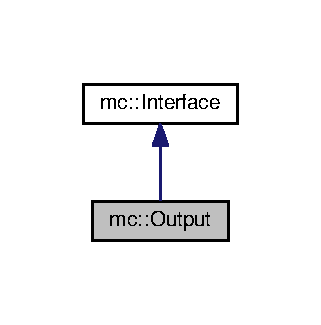
\includegraphics[width=154pt]{classmc_1_1Output__inherit__graph}
\end{center}
\end{figure}


Collaboration diagram for mc\+:\+:Output\+:\nopagebreak
\begin{figure}[H]
\begin{center}
\leavevmode
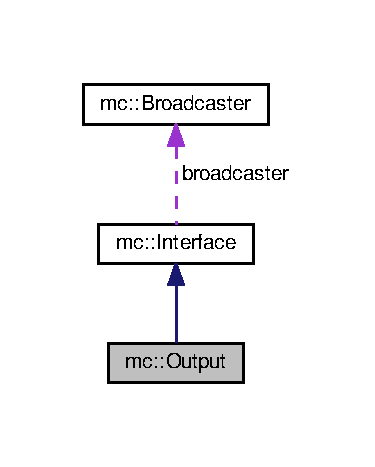
\includegraphics[width=180pt]{classmc_1_1Output__coll__graph}
\end{center}
\end{figure}
\subsection*{Public Member Functions}
\begin{DoxyCompactItemize}
\item 
\hyperlink{classmc_1_1Output_a5876f782da4e0412765ec6d00acafcfc}{Output} (Gtk\+::\+Label $\ast$w, \hyperlink{application_8hpp_ab701e3ac61a85b337ec5c1abaad6742d}{json} $\ast$d)
\item 
\hyperlink{classmc_1_1Output_a008a9b63a361317f496bfc321d5f3972}{$\sim$\+Output} ()
\item 
void \hyperlink{classmc_1_1Output_ac743a7671116432ddaf910e1ffb8eaa2}{notify} (\hyperlink{classmc_1_1Event}{Event} $\ast$e)
\item 
void \hyperlink{classmc_1_1Output_a4551a309472c048d9c5c14786cc623a1}{broadcast} ()
\item 
void \hyperlink{classmc_1_1Output_a6d84487fd991c839954d8458862d1aab}{set\+\_\+references} (std\+::vector$<$ \hyperlink{classmc_1_1Interface}{Interface} $\ast$ $>$ r)
\item 
void \hyperlink{classmc_1_1Output_a6953830b79ed5b8360b0fd4e0af50f19}{set\+\_\+calculator} (std\+::function$<$ double(std\+::vector$<$ \hyperlink{classmc_1_1Interface}{mc\+::\+Interface} $\ast$ $>$)$>$ f)
\item 
std\+::string \hyperlink{classmc_1_1Output_ab4ee892d21cd77e44f8c492e8ac62e99}{get\+\_\+value} ()
\item 
void \hyperlink{classmc_1_1Output_a49c49122555095cc88668a8af1aac944}{set\+\_\+value} (double v)
\end{DoxyCompactItemize}
\subsection*{Additional Inherited Members}


\subsection{Detailed Description}
The \hyperlink{classmc_1_1Output}{Output} class wraps a Gtk\+::\+Label in the UI and uses a provided lambda function to calculate a display value. 

\subsection{Constructor \& Destructor Documentation}
\index{mc\+::\+Output@{mc\+::\+Output}!Output@{Output}}
\index{Output@{Output}!mc\+::\+Output@{mc\+::\+Output}}
\subsubsection[{\texorpdfstring{Output(\+Gtk\+::\+Label $\ast$w, json $\ast$d)}{Output(Gtk::Label *w, json *d)}}]{\setlength{\rightskip}{0pt plus 5cm}mc\+::\+Output\+::\+Output (
\begin{DoxyParamCaption}
\item[{Gtk\+::\+Label $\ast$}]{w, }
\item[{{\bf json} $\ast$}]{d}
\end{DoxyParamCaption}
)}\hypertarget{classmc_1_1Output_a5876f782da4e0412765ec6d00acafcfc}{}\label{classmc_1_1Output_a5876f782da4e0412765ec6d00acafcfc}
Constructor 
\begin{DoxyParams}{Parameters}
{\em w} & the Gtk\+::\+Label to wrap \\
\hline
{\em d} & Pointer to the json datastore \\
\hline
\end{DoxyParams}
\index{mc\+::\+Output@{mc\+::\+Output}!````~Output@{$\sim$\+Output}}
\index{````~Output@{$\sim$\+Output}!mc\+::\+Output@{mc\+::\+Output}}
\subsubsection[{\texorpdfstring{$\sim$\+Output()}{~Output()}}]{\setlength{\rightskip}{0pt plus 5cm}mc\+::\+Output\+::$\sim$\+Output (
\begin{DoxyParamCaption}
{}
\end{DoxyParamCaption}
)}\hypertarget{classmc_1_1Output_a008a9b63a361317f496bfc321d5f3972}{}\label{classmc_1_1Output_a008a9b63a361317f496bfc321d5f3972}
Destructor 

\subsection{Member Function Documentation}
\index{mc\+::\+Output@{mc\+::\+Output}!broadcast@{broadcast}}
\index{broadcast@{broadcast}!mc\+::\+Output@{mc\+::\+Output}}
\subsubsection[{\texorpdfstring{broadcast()}{broadcast()}}]{\setlength{\rightskip}{0pt plus 5cm}void mc\+::\+Output\+::broadcast (
\begin{DoxyParamCaption}
{}
\end{DoxyParamCaption}
)\hspace{0.3cm}{\ttfamily [virtual]}}\hypertarget{classmc_1_1Output_a4551a309472c048d9c5c14786cc623a1}{}\label{classmc_1_1Output_a4551a309472c048d9c5c14786cc623a1}
Generates a change event and sends it to \hyperlink{classmc_1_1Broadcaster}{Broadcaster}. 

Implements \hyperlink{classmc_1_1Interface_af91ff5ec779e5af49bf798d5f6331b80}{mc\+::\+Interface}.

\index{mc\+::\+Output@{mc\+::\+Output}!get\+\_\+value@{get\+\_\+value}}
\index{get\+\_\+value@{get\+\_\+value}!mc\+::\+Output@{mc\+::\+Output}}
\subsubsection[{\texorpdfstring{get\+\_\+value()}{get_value()}}]{\setlength{\rightskip}{0pt plus 5cm}std\+::string mc\+::\+Output\+::get\+\_\+value (
\begin{DoxyParamCaption}
{}
\end{DoxyParamCaption}
)\hspace{0.3cm}{\ttfamily [virtual]}}\hypertarget{classmc_1_1Output_ab4ee892d21cd77e44f8c492e8ac62e99}{}\label{classmc_1_1Output_ab4ee892d21cd77e44f8c492e8ac62e99}
Returns a string representation of the current value of the \hyperlink{classmc_1_1Interface}{Interface}. 

Implements \hyperlink{classmc_1_1Interface_af8054c8af251199c9d142ce94182c5f5}{mc\+::\+Interface}.

\index{mc\+::\+Output@{mc\+::\+Output}!notify@{notify}}
\index{notify@{notify}!mc\+::\+Output@{mc\+::\+Output}}
\subsubsection[{\texorpdfstring{notify(\+Event $\ast$e)}{notify(Event *e)}}]{\setlength{\rightskip}{0pt plus 5cm}void mc\+::\+Output\+::notify (
\begin{DoxyParamCaption}
\item[{{\bf Event} $\ast$}]{e}
\end{DoxyParamCaption}
)\hspace{0.3cm}{\ttfamily [virtual]}}\hypertarget{classmc_1_1Output_ac743a7671116432ddaf910e1ffb8eaa2}{}\label{classmc_1_1Output_ac743a7671116432ddaf910e1ffb8eaa2}
Update the \hyperlink{classmc_1_1Interface}{Interface} about change events. Used by broadcaster. 
\begin{DoxyParams}{Parameters}
{\em e} & The event object \\
\hline
\end{DoxyParams}


Implements \hyperlink{classmc_1_1Interface_a6a08326bd2ad5d40fe0427e97cebfbb6}{mc\+::\+Interface}.

\index{mc\+::\+Output@{mc\+::\+Output}!set\+\_\+calculator@{set\+\_\+calculator}}
\index{set\+\_\+calculator@{set\+\_\+calculator}!mc\+::\+Output@{mc\+::\+Output}}
\subsubsection[{\texorpdfstring{set\+\_\+calculator(std\+::function$<$ double(std\+::vector$<$ mc\+::\+Interface $\ast$ $>$)$>$ f)}{set_calculator(std::function< double(std::vector< mc::Interface * >)> f)}}]{\setlength{\rightskip}{0pt plus 5cm}void mc\+::\+Output\+::set\+\_\+calculator (
\begin{DoxyParamCaption}
\item[{std\+::function$<$ double(std\+::vector$<$ {\bf mc\+::\+Interface} $\ast$ $>$)$>$}]{f}
\end{DoxyParamCaption}
)}\hypertarget{classmc_1_1Output_a6953830b79ed5b8360b0fd4e0af50f19}{}\label{classmc_1_1Output_a6953830b79ed5b8360b0fd4e0af50f19}
Set the calculating function that will be used to generate output given the current state of the references. 
\begin{DoxyParams}{Parameters}
{\em f} & A function that will be used to calculate output. \\
\hline
\end{DoxyParams}
\index{mc\+::\+Output@{mc\+::\+Output}!set\+\_\+references@{set\+\_\+references}}
\index{set\+\_\+references@{set\+\_\+references}!mc\+::\+Output@{mc\+::\+Output}}
\subsubsection[{\texorpdfstring{set\+\_\+references(std\+::vector$<$ Interface $\ast$ $>$ r)}{set_references(std::vector< Interface * > r)}}]{\setlength{\rightskip}{0pt plus 5cm}void mc\+::\+Output\+::set\+\_\+references (
\begin{DoxyParamCaption}
\item[{std\+::vector$<$ {\bf Interface} $\ast$ $>$}]{r}
\end{DoxyParamCaption}
)}\hypertarget{classmc_1_1Output_a6d84487fd991c839954d8458862d1aab}{}\label{classmc_1_1Output_a6d84487fd991c839954d8458862d1aab}
Add references to the interface that will trigger the \hyperlink{classmc_1_1Output}{Output} to update when they change. 
\begin{DoxyParams}{Parameters}
{\em r} & A vector of Interfaces to use as a reference \\
\hline
\end{DoxyParams}
\index{mc\+::\+Output@{mc\+::\+Output}!set\+\_\+value@{set\+\_\+value}}
\index{set\+\_\+value@{set\+\_\+value}!mc\+::\+Output@{mc\+::\+Output}}
\subsubsection[{\texorpdfstring{set\+\_\+value(double v)}{set_value(double v)}}]{\setlength{\rightskip}{0pt plus 5cm}void mc\+::\+Output\+::set\+\_\+value (
\begin{DoxyParamCaption}
\item[{double}]{v}
\end{DoxyParamCaption}
)}\hypertarget{classmc_1_1Output_a49c49122555095cc88668a8af1aac944}{}\label{classmc_1_1Output_a49c49122555095cc88668a8af1aac944}
Sets the value of the output. 
\begin{DoxyParams}{Parameters}
{\em v} & A double value to set in the ui. \\
\hline
\end{DoxyParams}


The documentation for this class was generated from the following files\+:\begin{DoxyCompactItemize}
\item 
inc/\hyperlink{output_8hpp}{output.\+hpp}\item 
src/output.\+cpp\end{DoxyCompactItemize}

\hypertarget{classmc_1_1Slider}{}\section{mc\+:\+:Slider Class Reference}
\label{classmc_1_1Slider}\index{mc\+::\+Slider@{mc\+::\+Slider}}


{\ttfamily \#include $<$slider.\+hpp$>$}



Inheritance diagram for mc\+:\+:Slider\+:\nopagebreak
\begin{figure}[H]
\begin{center}
\leavevmode
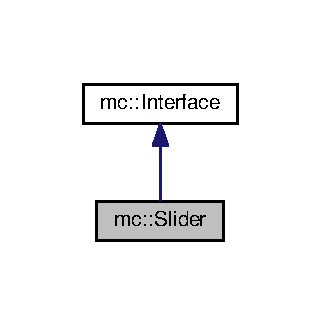
\includegraphics[width=154pt]{classmc_1_1Slider__inherit__graph}
\end{center}
\end{figure}


Collaboration diagram for mc\+:\+:Slider\+:\nopagebreak
\begin{figure}[H]
\begin{center}
\leavevmode
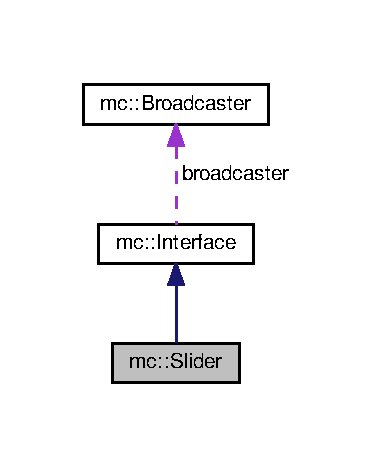
\includegraphics[width=180pt]{classmc_1_1Slider__coll__graph}
\end{center}
\end{figure}
\subsection*{Public Member Functions}
\begin{DoxyCompactItemize}
\item 
\hyperlink{classmc_1_1Slider_a33108d518cb39644076f6ca93f68ea4b}{Slider} (Gtk\+::\+Scale $\ast$w, \hyperlink{application_8hpp_ab701e3ac61a85b337ec5c1abaad6742d}{json} $\ast$d)
\item 
\hyperlink{classmc_1_1Slider_afde5e7b53d80e8667111d36099ba7297}{$\sim$\+Slider} ()
\item 
void \hyperlink{classmc_1_1Slider_af846178478b713ca0b04d2185aa337ba}{notify} (\hyperlink{classmc_1_1Event}{Event} $\ast$e)
\item 
void \hyperlink{classmc_1_1Slider_aa9d5bfade889ea320f0b51c98695a4bb}{broadcast} ()
\item 
void \hyperlink{classmc_1_1Slider_a42c9a7dc4cc7db0098f6a8e1313ae098}{populate} ()
\item 
void \hyperlink{classmc_1_1Slider_a4b2ebc10a9ea97fa6eeecf94607e0f34}{set\+\_\+marks} ()
\item 
void \hyperlink{classmc_1_1Slider_a3f205ea7c86933d51bd66388cbbcfd02}{set\+\_\+marks} (std\+::map$<$ double, std\+::string $>$ m)
\item 
void \hyperlink{classmc_1_1Slider_a8c42b47ca7a322012ca2d8e0942cd69e}{set\+\_\+scaler} (\hyperlink{classmc_1_1Interface}{Interface} $\ast$i)
\item 
void \hyperlink{classmc_1_1Slider_afb09c7ce8ac735c70515dee677d20d73}{set\+\_\+references} (std\+::vector$<$ \hyperlink{classmc_1_1Interface}{Interface} $\ast$ $>$ s, std\+::vector$<$ \hyperlink{classmc_1_1Interface}{Interface} $\ast$ $>$ e)
\item 
std\+::string \hyperlink{classmc_1_1Slider_a115495fc20368a6b8df56be831056cc3}{get\+\_\+value} ()
\item 
void \hyperlink{classmc_1_1Slider_a720804ffc2f064836538e2a21e38f3b3}{set\+\_\+value} (double max, double min, double val)
\end{DoxyCompactItemize}
\subsection*{Additional Inherited Members}


\subsection{Detailed Description}
A \hyperlink{classmc_1_1Slider}{Slider} wraps a Gtk\+::\+Scale widget in the UI and manages flexible max/min values, responding to broadcast events. 

\subsection{Constructor \& Destructor Documentation}
\index{mc\+::\+Slider@{mc\+::\+Slider}!Slider@{Slider}}
\index{Slider@{Slider}!mc\+::\+Slider@{mc\+::\+Slider}}
\subsubsection[{\texorpdfstring{Slider(\+Gtk\+::\+Scale $\ast$w, json $\ast$d)}{Slider(Gtk::Scale *w, json *d)}}]{\setlength{\rightskip}{0pt plus 5cm}mc\+::\+Slider\+::\+Slider (
\begin{DoxyParamCaption}
\item[{Gtk\+::\+Scale $\ast$}]{w, }
\item[{{\bf json} $\ast$}]{d}
\end{DoxyParamCaption}
)}\hypertarget{classmc_1_1Slider_a33108d518cb39644076f6ca93f68ea4b}{}\label{classmc_1_1Slider_a33108d518cb39644076f6ca93f68ea4b}
Constructor 
\begin{DoxyParams}{Parameters}
{\em w} & the Gtk\+::\+Label to wrap \\
\hline
{\em d} & Pointer to the json datastore \\
\hline
\end{DoxyParams}
\index{mc\+::\+Slider@{mc\+::\+Slider}!````~Slider@{$\sim$\+Slider}}
\index{````~Slider@{$\sim$\+Slider}!mc\+::\+Slider@{mc\+::\+Slider}}
\subsubsection[{\texorpdfstring{$\sim$\+Slider()}{~Slider()}}]{\setlength{\rightskip}{0pt plus 5cm}mc\+::\+Slider\+::$\sim$\+Slider (
\begin{DoxyParamCaption}
{}
\end{DoxyParamCaption}
)}\hypertarget{classmc_1_1Slider_afde5e7b53d80e8667111d36099ba7297}{}\label{classmc_1_1Slider_afde5e7b53d80e8667111d36099ba7297}
Destructor 

\subsection{Member Function Documentation}
\index{mc\+::\+Slider@{mc\+::\+Slider}!broadcast@{broadcast}}
\index{broadcast@{broadcast}!mc\+::\+Slider@{mc\+::\+Slider}}
\subsubsection[{\texorpdfstring{broadcast()}{broadcast()}}]{\setlength{\rightskip}{0pt plus 5cm}void mc\+::\+Slider\+::broadcast (
\begin{DoxyParamCaption}
{}
\end{DoxyParamCaption}
)\hspace{0.3cm}{\ttfamily [virtual]}}\hypertarget{classmc_1_1Slider_aa9d5bfade889ea320f0b51c98695a4bb}{}\label{classmc_1_1Slider_aa9d5bfade889ea320f0b51c98695a4bb}
Generates a change event and sends it to \hyperlink{classmc_1_1Broadcaster}{Broadcaster}. 

Implements \hyperlink{classmc_1_1Interface_af91ff5ec779e5af49bf798d5f6331b80}{mc\+::\+Interface}.

\index{mc\+::\+Slider@{mc\+::\+Slider}!get\+\_\+value@{get\+\_\+value}}
\index{get\+\_\+value@{get\+\_\+value}!mc\+::\+Slider@{mc\+::\+Slider}}
\subsubsection[{\texorpdfstring{get\+\_\+value()}{get_value()}}]{\setlength{\rightskip}{0pt plus 5cm}std\+::string mc\+::\+Slider\+::get\+\_\+value (
\begin{DoxyParamCaption}
{}
\end{DoxyParamCaption}
)\hspace{0.3cm}{\ttfamily [virtual]}}\hypertarget{classmc_1_1Slider_a115495fc20368a6b8df56be831056cc3}{}\label{classmc_1_1Slider_a115495fc20368a6b8df56be831056cc3}
Returns a string representation of the current value of the \hyperlink{classmc_1_1Interface}{Interface}. 

Implements \hyperlink{classmc_1_1Interface_af8054c8af251199c9d142ce94182c5f5}{mc\+::\+Interface}.

\index{mc\+::\+Slider@{mc\+::\+Slider}!notify@{notify}}
\index{notify@{notify}!mc\+::\+Slider@{mc\+::\+Slider}}
\subsubsection[{\texorpdfstring{notify(\+Event $\ast$e)}{notify(Event *e)}}]{\setlength{\rightskip}{0pt plus 5cm}void mc\+::\+Slider\+::notify (
\begin{DoxyParamCaption}
\item[{{\bf Event} $\ast$}]{e}
\end{DoxyParamCaption}
)\hspace{0.3cm}{\ttfamily [virtual]}}\hypertarget{classmc_1_1Slider_af846178478b713ca0b04d2185aa337ba}{}\label{classmc_1_1Slider_af846178478b713ca0b04d2185aa337ba}
Update the \hyperlink{classmc_1_1Interface}{Interface} about change events. Used by broadcaster. 
\begin{DoxyParams}{Parameters}
{\em e} & The event object \\
\hline
\end{DoxyParams}


Implements \hyperlink{classmc_1_1Interface_a6a08326bd2ad5d40fe0427e97cebfbb6}{mc\+::\+Interface}.

\index{mc\+::\+Slider@{mc\+::\+Slider}!populate@{populate}}
\index{populate@{populate}!mc\+::\+Slider@{mc\+::\+Slider}}
\subsubsection[{\texorpdfstring{populate()}{populate()}}]{\setlength{\rightskip}{0pt plus 5cm}void mc\+::\+Slider\+::populate (
\begin{DoxyParamCaption}
{}
\end{DoxyParamCaption}
)}\hypertarget{classmc_1_1Slider_a42c9a7dc4cc7db0098f6a8e1313ae098}{}\label{classmc_1_1Slider_a42c9a7dc4cc7db0098f6a8e1313ae098}
Populates the UI with values from the datastore. \index{mc\+::\+Slider@{mc\+::\+Slider}!set\+\_\+marks@{set\+\_\+marks}}
\index{set\+\_\+marks@{set\+\_\+marks}!mc\+::\+Slider@{mc\+::\+Slider}}
\subsubsection[{\texorpdfstring{set\+\_\+marks()}{set_marks()}}]{\setlength{\rightskip}{0pt plus 5cm}void mc\+::\+Slider\+::set\+\_\+marks (
\begin{DoxyParamCaption}
{}
\end{DoxyParamCaption}
)}\hypertarget{classmc_1_1Slider_a4b2ebc10a9ea97fa6eeecf94607e0f34}{}\label{classmc_1_1Slider_a4b2ebc10a9ea97fa6eeecf94607e0f34}
Sets any marks that this \hyperlink{classmc_1_1Slider}{Slider} contains in the UI. \index{mc\+::\+Slider@{mc\+::\+Slider}!set\+\_\+marks@{set\+\_\+marks}}
\index{set\+\_\+marks@{set\+\_\+marks}!mc\+::\+Slider@{mc\+::\+Slider}}
\subsubsection[{\texorpdfstring{set\+\_\+marks(std\+::map$<$ double, std\+::string $>$ m)}{set_marks(std::map< double, std::string > m)}}]{\setlength{\rightskip}{0pt plus 5cm}void mc\+::\+Slider\+::set\+\_\+marks (
\begin{DoxyParamCaption}
\item[{std\+::map$<$ double, std\+::string $>$}]{m}
\end{DoxyParamCaption}
)}\hypertarget{classmc_1_1Slider_a3f205ea7c86933d51bd66388cbbcfd02}{}\label{classmc_1_1Slider_a3f205ea7c86933d51bd66388cbbcfd02}
Overloaded set\+\_\+marks is used to provide constant mark values to add to the Gtk\+::\+Scale. 
\begin{DoxyParams}{Parameters}
{\em m} & A map of double (position) and string (label) values. \\
\hline
\end{DoxyParams}
\index{mc\+::\+Slider@{mc\+::\+Slider}!set\+\_\+references@{set\+\_\+references}}
\index{set\+\_\+references@{set\+\_\+references}!mc\+::\+Slider@{mc\+::\+Slider}}
\subsubsection[{\texorpdfstring{set\+\_\+references(std\+::vector$<$ Interface $\ast$ $>$ s, std\+::vector$<$ Interface $\ast$ $>$ e)}{set_references(std::vector< Interface * > s, std::vector< Interface * > e)}}]{\setlength{\rightskip}{0pt plus 5cm}void mc\+::\+Slider\+::set\+\_\+references (
\begin{DoxyParamCaption}
\item[{std\+::vector$<$ {\bf Interface} $\ast$ $>$}]{s, }
\item[{std\+::vector$<$ {\bf Interface} $\ast$ $>$}]{e}
\end{DoxyParamCaption}
)}\hypertarget{classmc_1_1Slider_afb09c7ce8ac735c70515dee677d20d73}{}\label{classmc_1_1Slider_afb09c7ce8ac735c70515dee677d20d73}
Add references to the interface that will trigger the \hyperlink{classmc_1_1Slider}{Slider} to update. \hyperlink{classmc_1_1Slider}{Slider} uses two sets of references and a scaler value to move the available range of values between the two.


\begin{DoxyParams}{Parameters}
{\em s} & A vector of Interfaces to use as a reference \\
\hline
{\em e} & A vector of Interfaces to use as a reference \\
\hline
\end{DoxyParams}
\index{mc\+::\+Slider@{mc\+::\+Slider}!set\+\_\+scaler@{set\+\_\+scaler}}
\index{set\+\_\+scaler@{set\+\_\+scaler}!mc\+::\+Slider@{mc\+::\+Slider}}
\subsubsection[{\texorpdfstring{set\+\_\+scaler(\+Interface $\ast$i)}{set_scaler(Interface *i)}}]{\setlength{\rightskip}{0pt plus 5cm}void mc\+::\+Slider\+::set\+\_\+scaler (
\begin{DoxyParamCaption}
\item[{{\bf Interface} $\ast$}]{i}
\end{DoxyParamCaption}
)}\hypertarget{classmc_1_1Slider_a8c42b47ca7a322012ca2d8e0942cd69e}{}\label{classmc_1_1Slider_a8c42b47ca7a322012ca2d8e0942cd69e}
The scaler is an \hyperlink{classmc_1_1Interface}{Interface} that is expected to be a value between 0-\/100 and is used to change the max and min values of this slider. 
\begin{DoxyParams}{Parameters}
{\em i} & The \hyperlink{classmc_1_1Interface}{Interface} to use as a scaler. \\
\hline
\end{DoxyParams}
\index{mc\+::\+Slider@{mc\+::\+Slider}!set\+\_\+value@{set\+\_\+value}}
\index{set\+\_\+value@{set\+\_\+value}!mc\+::\+Slider@{mc\+::\+Slider}}
\subsubsection[{\texorpdfstring{set\+\_\+value(double max, double min, double val)}{set_value(double max, double min, double val)}}]{\setlength{\rightskip}{0pt plus 5cm}void mc\+::\+Slider\+::set\+\_\+value (
\begin{DoxyParamCaption}
\item[{double}]{max, }
\item[{double}]{min, }
\item[{double}]{val}
\end{DoxyParamCaption}
)}\hypertarget{classmc_1_1Slider_a720804ffc2f064836538e2a21e38f3b3}{}\label{classmc_1_1Slider_a720804ffc2f064836538e2a21e38f3b3}
Sets the max, min and current position of the \hyperlink{classmc_1_1Slider}{Slider}. 

The documentation for this class was generated from the following files\+:\begin{DoxyCompactItemize}
\item 
inc/\hyperlink{slider_8hpp}{slider.\+hpp}\item 
src/slider.\+cpp\end{DoxyCompactItemize}

\hypertarget{classmc_1_1Spinner}{}\section{mc\+:\+:Spinner Class Reference}
\label{classmc_1_1Spinner}\index{mc\+::\+Spinner@{mc\+::\+Spinner}}


{\ttfamily \#include $<$spinner.\+hpp$>$}



Inheritance diagram for mc\+:\+:Spinner\+:\nopagebreak
\begin{figure}[H]
\begin{center}
\leavevmode
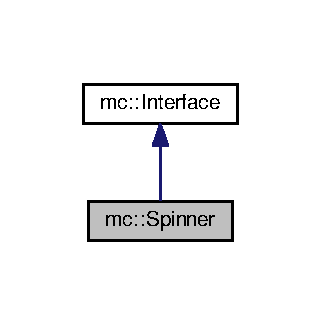
\includegraphics[width=154pt]{classmc_1_1Spinner__inherit__graph}
\end{center}
\end{figure}


Collaboration diagram for mc\+:\+:Spinner\+:\nopagebreak
\begin{figure}[H]
\begin{center}
\leavevmode
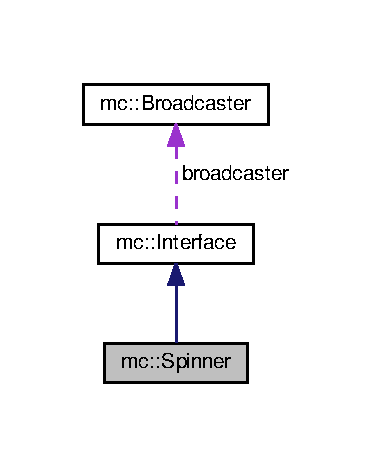
\includegraphics[width=180pt]{classmc_1_1Spinner__coll__graph}
\end{center}
\end{figure}
\subsection*{Public Member Functions}
\begin{DoxyCompactItemize}
\item 
\hyperlink{classmc_1_1Spinner_a96d963ce40e54531912178afc95ba9a5}{Spinner} (Gtk\+::\+Spin\+Button $\ast$w, \hyperlink{application_8hpp_ab701e3ac61a85b337ec5c1abaad6742d}{json} $\ast$d)
\item 
\hyperlink{classmc_1_1Spinner_a6e9f8cdd594f84e5a58d96c40de9c3aa}{$\sim$\+Spinner} ()
\item 
void \hyperlink{classmc_1_1Spinner_af3efb6a9cec2d6e3bfdb85f2cc88b0be}{notify} (\hyperlink{classmc_1_1Event}{Event} $\ast$e)
\item 
void \hyperlink{classmc_1_1Spinner_a6709da2aec22fdd2d8d19679c0f60762}{broadcast} ()
\item 
void \hyperlink{classmc_1_1Spinner_aec39936ffbdebb33a016d5ec5b681ddb}{set\+\_\+references} (std\+::vector$<$ \hyperlink{classmc_1_1Interface}{Interface} $\ast$ $>$ r)
\item 
std\+::string \hyperlink{classmc_1_1Spinner_a4675ce29a95e79138dd209ef6af5607d}{get\+\_\+value} ()
\item 
void \hyperlink{classmc_1_1Spinner_a07b81c140918785ac424222634ef4b03}{set\+\_\+value} (double d)
\end{DoxyCompactItemize}
\subsection*{Additional Inherited Members}


\subsection{Detailed Description}
A wrapper around a Gtk\+::\+Spinbutton. 

\subsection{Constructor \& Destructor Documentation}
\index{mc\+::\+Spinner@{mc\+::\+Spinner}!Spinner@{Spinner}}
\index{Spinner@{Spinner}!mc\+::\+Spinner@{mc\+::\+Spinner}}
\subsubsection[{\texorpdfstring{Spinner(\+Gtk\+::\+Spin\+Button $\ast$w, json $\ast$d)}{Spinner(Gtk::SpinButton *w, json *d)}}]{\setlength{\rightskip}{0pt plus 5cm}mc\+::\+Spinner\+::\+Spinner (
\begin{DoxyParamCaption}
\item[{Gtk\+::\+Spin\+Button $\ast$}]{w, }
\item[{{\bf json} $\ast$}]{d}
\end{DoxyParamCaption}
)}\hypertarget{classmc_1_1Spinner_a96d963ce40e54531912178afc95ba9a5}{}\label{classmc_1_1Spinner_a96d963ce40e54531912178afc95ba9a5}
Constructor 
\begin{DoxyParams}{Parameters}
{\em w} & the Gtk\+::\+Spin\+Button to wrap \\
\hline
{\em d} & Pointer to the json datastore \\
\hline
\end{DoxyParams}
\index{mc\+::\+Spinner@{mc\+::\+Spinner}!````~Spinner@{$\sim$\+Spinner}}
\index{````~Spinner@{$\sim$\+Spinner}!mc\+::\+Spinner@{mc\+::\+Spinner}}
\subsubsection[{\texorpdfstring{$\sim$\+Spinner()}{~Spinner()}}]{\setlength{\rightskip}{0pt plus 5cm}mc\+::\+Spinner\+::$\sim$\+Spinner (
\begin{DoxyParamCaption}
{}
\end{DoxyParamCaption}
)}\hypertarget{classmc_1_1Spinner_a6e9f8cdd594f84e5a58d96c40de9c3aa}{}\label{classmc_1_1Spinner_a6e9f8cdd594f84e5a58d96c40de9c3aa}
Destructor 

\subsection{Member Function Documentation}
\index{mc\+::\+Spinner@{mc\+::\+Spinner}!broadcast@{broadcast}}
\index{broadcast@{broadcast}!mc\+::\+Spinner@{mc\+::\+Spinner}}
\subsubsection[{\texorpdfstring{broadcast()}{broadcast()}}]{\setlength{\rightskip}{0pt plus 5cm}void mc\+::\+Spinner\+::broadcast (
\begin{DoxyParamCaption}
{}
\end{DoxyParamCaption}
)\hspace{0.3cm}{\ttfamily [virtual]}}\hypertarget{classmc_1_1Spinner_a6709da2aec22fdd2d8d19679c0f60762}{}\label{classmc_1_1Spinner_a6709da2aec22fdd2d8d19679c0f60762}
Generates a change event and sends it to \hyperlink{classmc_1_1Broadcaster}{Broadcaster}. 

Implements \hyperlink{classmc_1_1Interface_af91ff5ec779e5af49bf798d5f6331b80}{mc\+::\+Interface}.

\index{mc\+::\+Spinner@{mc\+::\+Spinner}!get\+\_\+value@{get\+\_\+value}}
\index{get\+\_\+value@{get\+\_\+value}!mc\+::\+Spinner@{mc\+::\+Spinner}}
\subsubsection[{\texorpdfstring{get\+\_\+value()}{get_value()}}]{\setlength{\rightskip}{0pt plus 5cm}std\+::string mc\+::\+Spinner\+::get\+\_\+value (
\begin{DoxyParamCaption}
{}
\end{DoxyParamCaption}
)\hspace{0.3cm}{\ttfamily [virtual]}}\hypertarget{classmc_1_1Spinner_a4675ce29a95e79138dd209ef6af5607d}{}\label{classmc_1_1Spinner_a4675ce29a95e79138dd209ef6af5607d}
Returns a string representation of the current value of the \hyperlink{classmc_1_1Spinner}{Spinner}. 

Implements \hyperlink{classmc_1_1Interface_af8054c8af251199c9d142ce94182c5f5}{mc\+::\+Interface}.

\index{mc\+::\+Spinner@{mc\+::\+Spinner}!notify@{notify}}
\index{notify@{notify}!mc\+::\+Spinner@{mc\+::\+Spinner}}
\subsubsection[{\texorpdfstring{notify(\+Event $\ast$e)}{notify(Event *e)}}]{\setlength{\rightskip}{0pt plus 5cm}void mc\+::\+Spinner\+::notify (
\begin{DoxyParamCaption}
\item[{{\bf Event} $\ast$}]{e}
\end{DoxyParamCaption}
)\hspace{0.3cm}{\ttfamily [virtual]}}\hypertarget{classmc_1_1Spinner_af3efb6a9cec2d6e3bfdb85f2cc88b0be}{}\label{classmc_1_1Spinner_af3efb6a9cec2d6e3bfdb85f2cc88b0be}
Update the \hyperlink{classmc_1_1Interface}{Interface} about change events. Used by broadcaster. 
\begin{DoxyParams}{Parameters}
{\em e} & The event object \\
\hline
\end{DoxyParams}


Implements \hyperlink{classmc_1_1Interface_a6a08326bd2ad5d40fe0427e97cebfbb6}{mc\+::\+Interface}.

\index{mc\+::\+Spinner@{mc\+::\+Spinner}!set\+\_\+references@{set\+\_\+references}}
\index{set\+\_\+references@{set\+\_\+references}!mc\+::\+Spinner@{mc\+::\+Spinner}}
\subsubsection[{\texorpdfstring{set\+\_\+references(std\+::vector$<$ Interface $\ast$ $>$ r)}{set_references(std::vector< Interface * > r)}}]{\setlength{\rightskip}{0pt plus 5cm}void mc\+::\+Spinner\+::set\+\_\+references (
\begin{DoxyParamCaption}
\item[{std\+::vector$<$ {\bf Interface} $\ast$ $>$}]{r}
\end{DoxyParamCaption}
)}\hypertarget{classmc_1_1Spinner_aec39936ffbdebb33a016d5ec5b681ddb}{}\label{classmc_1_1Spinner_aec39936ffbdebb33a016d5ec5b681ddb}
Add references to the interface that will trigger the \hyperlink{classmc_1_1Spinner}{Spinner} to update when they change. 
\begin{DoxyParams}{Parameters}
{\em r} & A vector of Interfaces to use as a reference \\
\hline
\end{DoxyParams}
\index{mc\+::\+Spinner@{mc\+::\+Spinner}!set\+\_\+value@{set\+\_\+value}}
\index{set\+\_\+value@{set\+\_\+value}!mc\+::\+Spinner@{mc\+::\+Spinner}}
\subsubsection[{\texorpdfstring{set\+\_\+value(double d)}{set_value(double d)}}]{\setlength{\rightskip}{0pt plus 5cm}void mc\+::\+Spinner\+::set\+\_\+value (
\begin{DoxyParamCaption}
\item[{double}]{d}
\end{DoxyParamCaption}
)}\hypertarget{classmc_1_1Spinner_a07b81c140918785ac424222634ef4b03}{}\label{classmc_1_1Spinner_a07b81c140918785ac424222634ef4b03}
Sets the current value of the \hyperlink{classmc_1_1Spinner}{Spinner}.. 

The documentation for this class was generated from the following files\+:\begin{DoxyCompactItemize}
\item 
inc/\hyperlink{spinner_8hpp}{spinner.\+hpp}\item 
src/spinner.\+cpp\end{DoxyCompactItemize}

\chapter{File Documentation}
\hypertarget{application_8hpp}{}\section{inc/application.hpp File Reference}
\label{application_8hpp}\index{inc/application.\+hpp@{inc/application.\+hpp}}


The class definition file for the main application class.  


{\ttfamily \#include $<$map$>$}\\*
{\ttfamily \#include $<$gtkmm.\+h$>$}\\*
{\ttfamily \#include \char`\"{}json.\+hpp\char`\"{}}\\*
Include dependency graph for application.\+hpp\+:\nopagebreak
\begin{figure}[H]
\begin{center}
\leavevmode
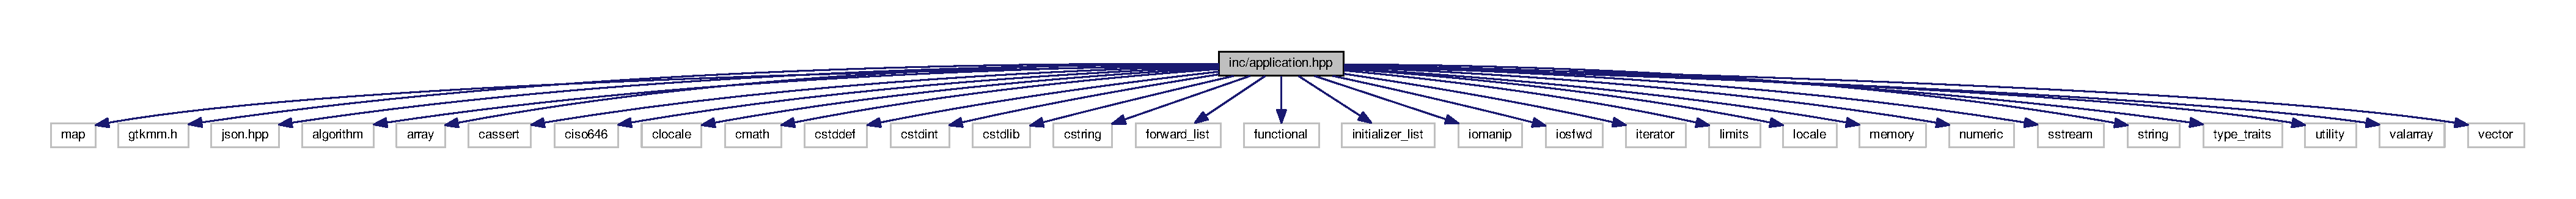
\includegraphics[width=350pt]{application_8hpp__incl}
\end{center}
\end{figure}
This graph shows which files directly or indirectly include this file\+:\nopagebreak
\begin{figure}[H]
\begin{center}
\leavevmode
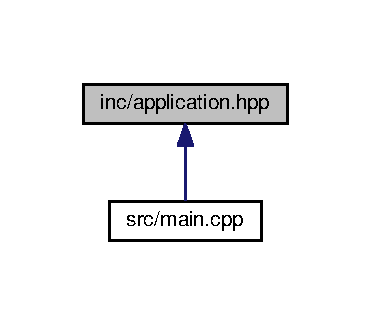
\includegraphics[width=178pt]{application_8hpp__dep__incl}
\end{center}
\end{figure}
\subsection*{Classes}
\begin{DoxyCompactItemize}
\item 
class \hyperlink{classmcalc_1_1Application}{mcalc\+::\+Application}
\end{DoxyCompactItemize}
\subsection*{Namespaces}
\begin{DoxyCompactItemize}
\item 
 \hyperlink{namespacemcalc}{mcalc}
\end{DoxyCompactItemize}
\subsection*{Typedefs}
\begin{DoxyCompactItemize}
\item 
using \hyperlink{application_8hpp_ab701e3ac61a85b337ec5c1abaad6742d}{json} = nlohmann\+::json
\end{DoxyCompactItemize}


\subsection{Detailed Description}
The class definition file for the main application class. 

Manages the software as a whole and initializes all of the widgets and the datastore.

\begin{DoxyAuthor}{Author}
Michael House 
\end{DoxyAuthor}
\begin{DoxyVersion}{Version}
0.\+1 10/19/17 
\end{DoxyVersion}


\subsection{Typedef Documentation}
\index{application.\+hpp@{application.\+hpp}!json@{json}}
\index{json@{json}!application.\+hpp@{application.\+hpp}}
\subsubsection[{\texorpdfstring{json}{json}}]{\setlength{\rightskip}{0pt plus 5cm}using {\bf json} =  nlohmann\+::json}\hypertarget{application_8hpp_ab701e3ac61a85b337ec5c1abaad6742d}{}\label{application_8hpp_ab701e3ac61a85b337ec5c1abaad6742d}
alias for the nlohmann namespace 
\hypertarget{broadcaster_8hpp}{}\section{inc/broadcaster.hpp File Reference}
\label{broadcaster_8hpp}\index{inc/broadcaster.\+hpp@{inc/broadcaster.\+hpp}}


The class definition file for the broadcaster class.  


{\ttfamily \#include $<$vector$>$}\\*
Include dependency graph for broadcaster.\+hpp\+:\nopagebreak
\begin{figure}[H]
\begin{center}
\leavevmode
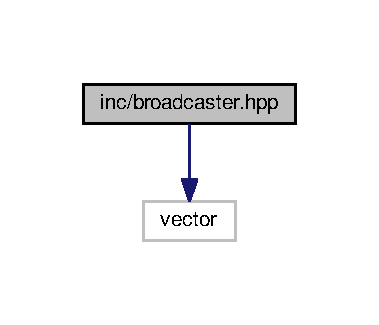
\includegraphics[width=182pt]{broadcaster_8hpp__incl}
\end{center}
\end{figure}
\subsection*{Classes}
\begin{DoxyCompactItemize}
\item 
class \hyperlink{classmc_1_1Broadcaster}{mc\+::\+Broadcaster}
\item 
class \hyperlink{classmc_1_1Event}{mc\+::\+Event}
\end{DoxyCompactItemize}


\subsection{Detailed Description}
The class definition file for the broadcaster class. 

Acts as a communication backbone for all interfaces, notifying all of them when one changes.

\begin{DoxyAuthor}{Author}
Michael House 
\end{DoxyAuthor}
\begin{DoxyVersion}{Version}
0.\+1 10/19/17 
\end{DoxyVersion}

\hypertarget{comboboxtext_8hpp}{}\section{inc/comboboxtext.hpp File Reference}
\label{comboboxtext_8hpp}\index{inc/comboboxtext.\+hpp@{inc/comboboxtext.\+hpp}}


The class definition file for the comboboxtext class.  


{\ttfamily \#include $<$vector$>$}\\*
{\ttfamily \#include $<$gtkmm.\+h$>$}\\*
{\ttfamily \#include \char`\"{}interface.\+hpp\char`\"{}}\\*
{\ttfamily \#include \char`\"{}json.\+hpp\char`\"{}}\\*
Include dependency graph for comboboxtext.\+hpp\+:\nopagebreak
\begin{figure}[H]
\begin{center}
\leavevmode
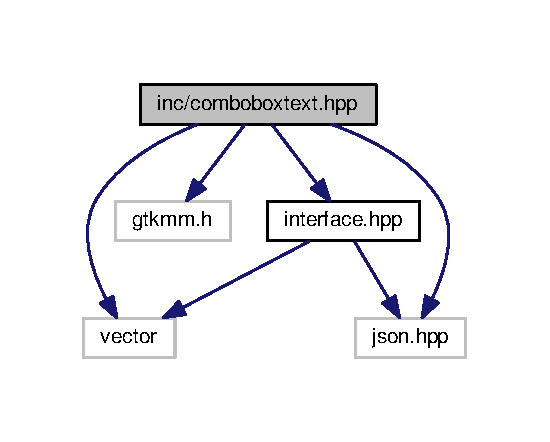
\includegraphics[width=264pt]{comboboxtext_8hpp__incl}
\end{center}
\end{figure}
\subsection*{Classes}
\begin{DoxyCompactItemize}
\item 
class \hyperlink{classmc_1_1ComboBoxText}{mc\+::\+Combo\+Box\+Text}
\end{DoxyCompactItemize}
\subsection*{Typedefs}
\begin{DoxyCompactItemize}
\item 
using \hyperlink{comboboxtext_8hpp_ab701e3ac61a85b337ec5c1abaad6742d}{json} = nlohmann\+::json
\end{DoxyCompactItemize}


\subsection{Detailed Description}
The class definition file for the comboboxtext class. 

Acts as a wrapper for a Gtk\+::\+Combo\+Box\+Text, broadcasting state changes and updating data in the combobox.

\begin{DoxyAuthor}{Author}
Michael House 
\end{DoxyAuthor}
\begin{DoxyVersion}{Version}
0.\+1 10/19/17 
\end{DoxyVersion}


\subsection{Typedef Documentation}
\index{comboboxtext.\+hpp@{comboboxtext.\+hpp}!json@{json}}
\index{json@{json}!comboboxtext.\+hpp@{comboboxtext.\+hpp}}
\subsubsection[{\texorpdfstring{json}{json}}]{\setlength{\rightskip}{0pt plus 5cm}using {\bf json} =  nlohmann\+::json}\hypertarget{comboboxtext_8hpp_ab701e3ac61a85b337ec5c1abaad6742d}{}\label{comboboxtext_8hpp_ab701e3ac61a85b337ec5c1abaad6742d}
alias for the nlohmann namespace 
\hypertarget{datastore_8hpp}{}\section{inc/datastore.hpp File Reference}
\label{datastore_8hpp}\index{inc/datastore.\+hpp@{inc/datastore.\+hpp}}


Contains generated data used by M\+Calc.  


{\ttfamily \#include $<$vector$>$}\\*
{\ttfamily \#include \char`\"{}json.\+hpp\char`\"{}}\\*
Include dependency graph for datastore.\+hpp\+:\nopagebreak
\begin{figure}[H]
\begin{center}
\leavevmode
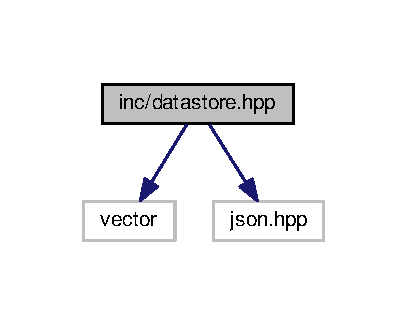
\includegraphics[width=196pt]{datastore_8hpp__incl}
\end{center}
\end{figure}
This graph shows which files directly or indirectly include this file\+:\nopagebreak
\begin{figure}[H]
\begin{center}
\leavevmode
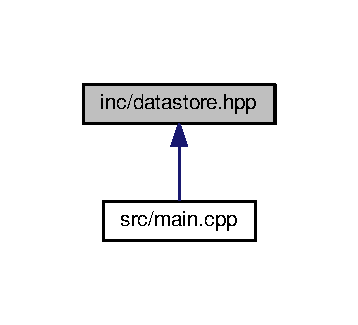
\includegraphics[width=172pt]{datastore_8hpp__dep__incl}
\end{center}
\end{figure}
\subsection*{Namespaces}
\begin{DoxyCompactItemize}
\item 
 \hyperlink{namespacemcalc}{mcalc}
\end{DoxyCompactItemize}
\subsection*{Typedefs}
\begin{DoxyCompactItemize}
\item 
using \hyperlink{datastore_8hpp_ab701e3ac61a85b337ec5c1abaad6742d}{json} = nlohmann\+::json
\end{DoxyCompactItemize}
\subsection*{Variables}
\begin{DoxyCompactItemize}
\item 
\hyperlink{application_8hpp_ab701e3ac61a85b337ec5c1abaad6742d}{json} \hyperlink{namespacemcalc_ae5e326e29d88ff26948cb46ed871e27f}{mcalc\+::material}
\end{DoxyCompactItemize}


\subsection{Detailed Description}
Contains generated data used by M\+Calc. 

The material J\+S\+ON object contains a large amount of data used by M\+Calc for lookups and calculations. It\textquotesingle{}s generated by a Python script.

\begin{DoxyAuthor}{Author}
Michael House 
\end{DoxyAuthor}
\begin{DoxyVersion}{Version}
0.\+1 10/19/17 
\end{DoxyVersion}


\subsection{Typedef Documentation}
\index{datastore.\+hpp@{datastore.\+hpp}!json@{json}}
\index{json@{json}!datastore.\+hpp@{datastore.\+hpp}}
\subsubsection[{\texorpdfstring{json}{json}}]{\setlength{\rightskip}{0pt plus 5cm}using {\bf json} =  nlohmann\+::json}\hypertarget{datastore_8hpp_ab701e3ac61a85b337ec5c1abaad6742d}{}\label{datastore_8hpp_ab701e3ac61a85b337ec5c1abaad6742d}
alias for the nlohmann namespace 
\hypertarget{interface_8hpp}{}\section{inc/interface.hpp File Reference}
\label{interface_8hpp}\index{inc/interface.\+hpp@{inc/interface.\+hpp}}


The class definition file for the interface abstract base class.  


{\ttfamily \#include $<$vector$>$}\\*
{\ttfamily \#include \char`\"{}json.\+hpp\char`\"{}}\\*
Include dependency graph for interface.\+hpp\+:\nopagebreak
\begin{figure}[H]
\begin{center}
\leavevmode
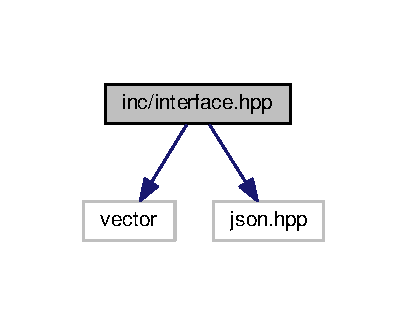
\includegraphics[width=196pt]{interface_8hpp__incl}
\end{center}
\end{figure}
This graph shows which files directly or indirectly include this file\+:\nopagebreak
\begin{figure}[H]
\begin{center}
\leavevmode
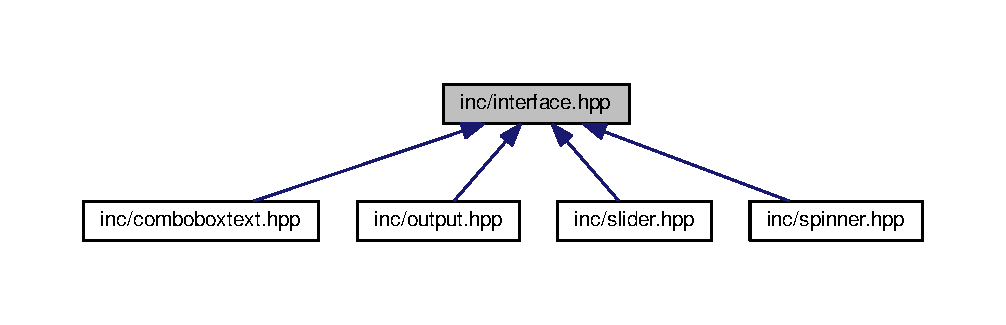
\includegraphics[width=350pt]{interface_8hpp__dep__incl}
\end{center}
\end{figure}
\subsection*{Classes}
\begin{DoxyCompactItemize}
\item 
class \hyperlink{classmc_1_1Interface}{mc\+::\+Interface}
\item 
class \hyperlink{classmc_1_1DummyInterface}{mc\+::\+Dummy\+Interface}
\end{DoxyCompactItemize}
\subsection*{Macros}
\begin{DoxyCompactItemize}
\item 
\#define \hyperlink{interface_8hpp_aa3da2a0fc67a48b3c131f0ff3d64f561}{\+\_\+vinterface}(V)~(new \hyperlink{classmc_1_1DummyInterface}{mc\+::\+Dummy\+Interface}(V))
\end{DoxyCompactItemize}
\subsection*{Typedefs}
\begin{DoxyCompactItemize}
\item 
using \hyperlink{interface_8hpp_ab701e3ac61a85b337ec5c1abaad6742d}{json} = nlohmann\+::json
\end{DoxyCompactItemize}


\subsection{Detailed Description}
The class definition file for the interface abstract base class. 

Acts as the base class of Combo\+Box\+Text, Slider, etc.

\begin{DoxyAuthor}{Author}
Michael House 
\end{DoxyAuthor}
\begin{DoxyVersion}{Version}
0.\+1 10/19/17 
\end{DoxyVersion}


\subsection{Macro Definition Documentation}
\index{interface.\+hpp@{interface.\+hpp}!\+\_\+vinterface@{\+\_\+vinterface}}
\index{\+\_\+vinterface@{\+\_\+vinterface}!interface.\+hpp@{interface.\+hpp}}
\subsubsection[{\texorpdfstring{\+\_\+vinterface}{_vinterface}}]{\setlength{\rightskip}{0pt plus 5cm}\#define \+\_\+vinterface(
\begin{DoxyParamCaption}
\item[{}]{V}
\end{DoxyParamCaption}
)~(new {\bf mc\+::\+Dummy\+Interface}(V))}\hypertarget{interface_8hpp_aa3da2a0fc67a48b3c131f0ff3d64f561}{}\label{interface_8hpp_aa3da2a0fc67a48b3c131f0ff3d64f561}
A macro to simplify the creation of a Dummy\+Interface 

\subsection{Typedef Documentation}
\index{interface.\+hpp@{interface.\+hpp}!json@{json}}
\index{json@{json}!interface.\+hpp@{interface.\+hpp}}
\subsubsection[{\texorpdfstring{json}{json}}]{\setlength{\rightskip}{0pt plus 5cm}using {\bf json} =  nlohmann\+::json}\hypertarget{interface_8hpp_ab701e3ac61a85b337ec5c1abaad6742d}{}\label{interface_8hpp_ab701e3ac61a85b337ec5c1abaad6742d}
alias for the nlohmann namespace 
\hypertarget{output_8hpp}{}\section{inc/output.hpp File Reference}
\label{output_8hpp}\index{inc/output.\+hpp@{inc/output.\+hpp}}


The class definition file for the output class.  


{\ttfamily \#include $<$vector$>$}\\*
{\ttfamily \#include $<$gtkmm.\+h$>$}\\*
{\ttfamily \#include \char`\"{}interface.\+hpp\char`\"{}}\\*
{\ttfamily \#include \char`\"{}json.\+hpp\char`\"{}}\\*
Include dependency graph for output.\+hpp\+:\nopagebreak
\begin{figure}[H]
\begin{center}
\leavevmode
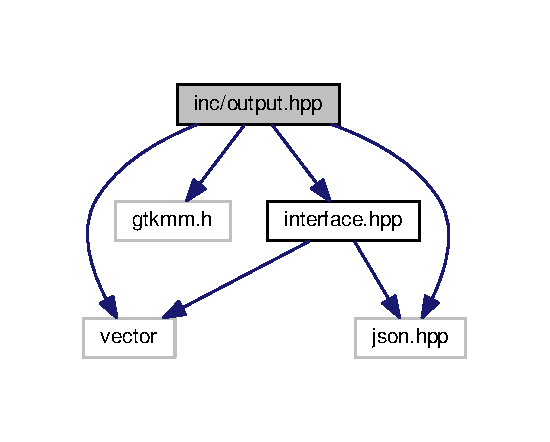
\includegraphics[width=264pt]{output_8hpp__incl}
\end{center}
\end{figure}
\subsection*{Classes}
\begin{DoxyCompactItemize}
\item 
class \hyperlink{classmc_1_1Output}{mc\+::\+Output}
\end{DoxyCompactItemize}
\subsection*{Typedefs}
\begin{DoxyCompactItemize}
\item 
using \hyperlink{output_8hpp_ab701e3ac61a85b337ec5c1abaad6742d}{json} = nlohmann\+::json
\end{DoxyCompactItemize}


\subsection{Detailed Description}
The class definition file for the output class. 

Acts as a wrapper for a Gtk\+::\+Label, updates the state and calculates output values.

\begin{DoxyAuthor}{Author}
Michael House 
\end{DoxyAuthor}
\begin{DoxyVersion}{Version}
0.\+1 10/19/17 
\end{DoxyVersion}


\subsection{Typedef Documentation}
\index{output.\+hpp@{output.\+hpp}!json@{json}}
\index{json@{json}!output.\+hpp@{output.\+hpp}}
\subsubsection[{\texorpdfstring{json}{json}}]{\setlength{\rightskip}{0pt plus 5cm}using {\bf json} =  nlohmann\+::json}\hypertarget{output_8hpp_ab701e3ac61a85b337ec5c1abaad6742d}{}\label{output_8hpp_ab701e3ac61a85b337ec5c1abaad6742d}
alias for the nlohmann namespace 
\hypertarget{slider_8hpp}{}\section{inc/slider.hpp File Reference}
\label{slider_8hpp}\index{inc/slider.\+hpp@{inc/slider.\+hpp}}


The class definition file for the slider class.  


{\ttfamily \#include $<$vector$>$}\\*
{\ttfamily \#include $<$gtkmm.\+h$>$}\\*
{\ttfamily \#include \char`\"{}interface.\+hpp\char`\"{}}\\*
{\ttfamily \#include \char`\"{}json.\+hpp\char`\"{}}\\*
Include dependency graph for slider.\+hpp\+:\nopagebreak
\begin{figure}[H]
\begin{center}
\leavevmode
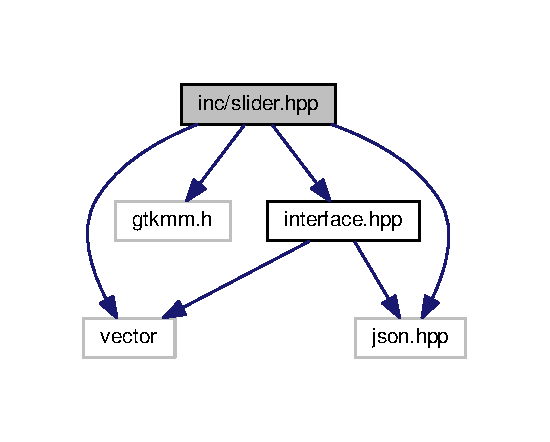
\includegraphics[width=264pt]{slider_8hpp__incl}
\end{center}
\end{figure}
\subsection*{Classes}
\begin{DoxyCompactItemize}
\item 
class \hyperlink{classmc_1_1Slider}{mc\+::\+Slider}
\end{DoxyCompactItemize}
\subsection*{Typedefs}
\begin{DoxyCompactItemize}
\item 
using \hyperlink{slider_8hpp_ab701e3ac61a85b337ec5c1abaad6742d}{json} = nlohmann\+::json
\end{DoxyCompactItemize}


\subsection{Detailed Description}
The class definition file for the slider class. 

Acts as a wrapper for a Gtk\+::\+Scale, updates the state and calculates max and min values.

\begin{DoxyAuthor}{Author}
Michael House 
\end{DoxyAuthor}
\begin{DoxyVersion}{Version}
0.\+1 10/19/17 
\end{DoxyVersion}


\subsection{Typedef Documentation}
\index{slider.\+hpp@{slider.\+hpp}!json@{json}}
\index{json@{json}!slider.\+hpp@{slider.\+hpp}}
\subsubsection[{\texorpdfstring{json}{json}}]{\setlength{\rightskip}{0pt plus 5cm}using {\bf json} =  nlohmann\+::json}\hypertarget{slider_8hpp_ab701e3ac61a85b337ec5c1abaad6742d}{}\label{slider_8hpp_ab701e3ac61a85b337ec5c1abaad6742d}
alias for the nlohmann namespace 
\hypertarget{spinner_8hpp}{}\section{inc/spinner.hpp File Reference}
\label{spinner_8hpp}\index{inc/spinner.\+hpp@{inc/spinner.\+hpp}}


The class definition file for the spinner class.  


{\ttfamily \#include $<$vector$>$}\\*
{\ttfamily \#include $<$gtkmm.\+h$>$}\\*
{\ttfamily \#include \char`\"{}interface.\+hpp\char`\"{}}\\*
{\ttfamily \#include \char`\"{}json.\+hpp\char`\"{}}\\*
Include dependency graph for spinner.\+hpp\+:\nopagebreak
\begin{figure}[H]
\begin{center}
\leavevmode
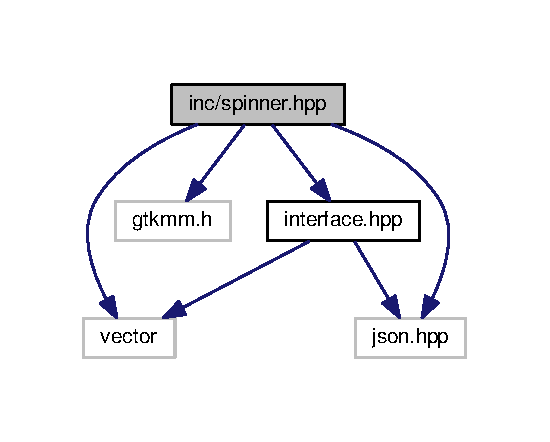
\includegraphics[width=264pt]{spinner_8hpp__incl}
\end{center}
\end{figure}
\subsection*{Classes}
\begin{DoxyCompactItemize}
\item 
class \hyperlink{classmc_1_1Spinner}{mc\+::\+Spinner}
\end{DoxyCompactItemize}
\subsection*{Typedefs}
\begin{DoxyCompactItemize}
\item 
using \hyperlink{spinner_8hpp_ab701e3ac61a85b337ec5c1abaad6742d}{json} = nlohmann\+::json
\end{DoxyCompactItemize}


\subsection{Detailed Description}
The class definition file for the spinner class. 

Acts as a wrapper for a Gtk\+::\+Spin\+Button, updates the state and broadcasts change events.

\begin{DoxyAuthor}{Author}
Michael House 
\end{DoxyAuthor}
\begin{DoxyVersion}{Version}
0.\+1 10/19/17 
\end{DoxyVersion}


\subsection{Typedef Documentation}
\index{spinner.\+hpp@{spinner.\+hpp}!json@{json}}
\index{json@{json}!spinner.\+hpp@{spinner.\+hpp}}
\subsubsection[{\texorpdfstring{json}{json}}]{\setlength{\rightskip}{0pt plus 5cm}using {\bf json} =  nlohmann\+::json}\hypertarget{spinner_8hpp_ab701e3ac61a85b337ec5c1abaad6742d}{}\label{spinner_8hpp_ab701e3ac61a85b337ec5c1abaad6742d}
alias for the nlohmann namespace 
\hypertarget{main_8cpp}{}\section{src/main.cpp File Reference}
\label{main_8cpp}\index{src/main.\+cpp@{src/main.\+cpp}}


This file contains the main function.  


{\ttfamily \#include $<$map$>$}\\*
{\ttfamily \#include $<$iostream$>$}\\*
{\ttfamily \#include $<$string$>$}\\*
{\ttfamily \#include $<$vector$>$}\\*
{\ttfamily \#include $<$gtkmm/builder.\+h$>$}\\*
{\ttfamily \#include \char`\"{}application.\+hpp\char`\"{}}\\*
{\ttfamily \#include \char`\"{}datastore.\+hpp\char`\"{}}\\*
Include dependency graph for main.\+cpp\+:\nopagebreak
\begin{figure}[H]
\begin{center}
\leavevmode
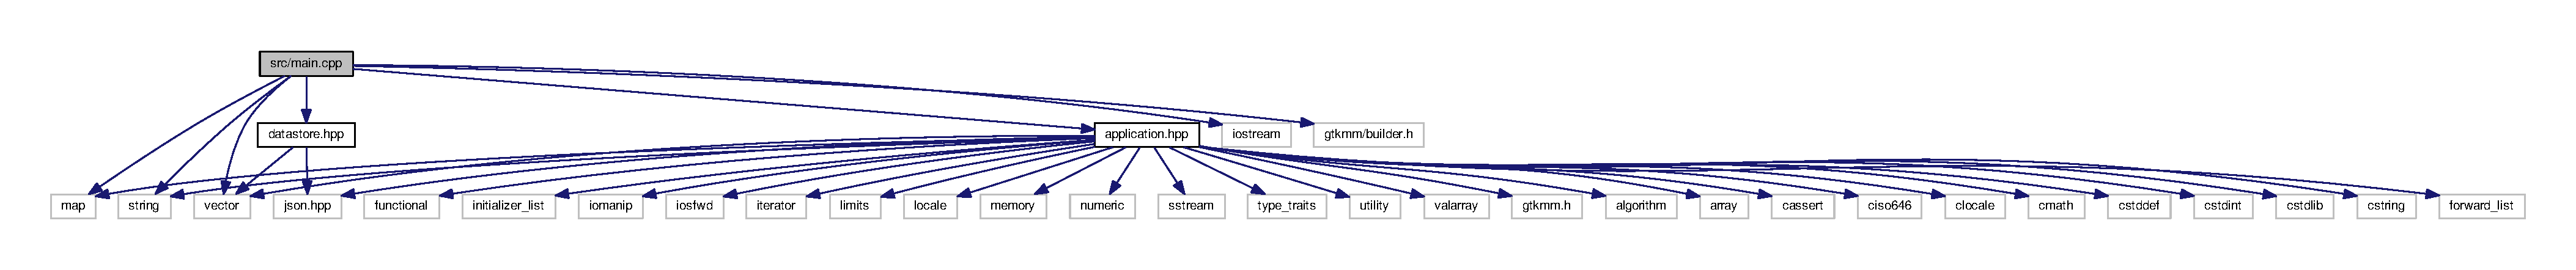
\includegraphics[width=350pt]{main_8cpp__incl}
\end{center}
\end{figure}
\subsection*{Functions}
\begin{DoxyCompactItemize}
\item 
int {\bfseries main} (int argc, char $\ast$argv\mbox{[}$\,$\mbox{]})\hypertarget{main_8cpp_a0ddf1224851353fc92bfbff6f499fa97}{}\label{main_8cpp_a0ddf1224851353fc92bfbff6f499fa97}

\end{DoxyCompactItemize}


\subsection{Detailed Description}
This file contains the main function. 

The main function initializes the Gtk\+::\+Application, loads the UI file (glade xml) and launches the \hyperlink{classmcalc_1_1Application}{mcalc\+::\+Application} to handle user interaction.

\begin{DoxyAuthor}{Author}
Michael House 
\end{DoxyAuthor}
\begin{DoxyVersion}{Version}
0.\+1 10/19/17 
\end{DoxyVersion}

%--- End generated contents ---

% Index
\backmatter
\newpage
\phantomsection
\clearemptydoublepage
\addcontentsline{toc}{chapter}{Index}
\printindex

\end{document}
